%%%%%%%%%%%%%%%%%%%%%%%%%%%%%%%%%%%%%%%%%%%%%%%%%%%
% conf-comandos.sty
%%%%%%%%%%%%%%%%%%%%%%%%%%%%%%%%%%%%%%%%%%%%%%%%%%%
	
\ProvidesPackage{conf-comandos}

% ----------------------------------------------------------
% Imprimir a ficha catalográfica
% ----------------------------------------------------------
\newcommand{\imprimirficha}[1]{
    \begin{fichacatalografica}
        \includepdf{#1}
    \end{fichacatalografica}
}

% ----------------------------------------------------------
% Imprimir a folha de aprovação
% ----------------------------------------------------------
 %\providecommand{\imprimirtextoaprovacao}{}
% \newcommand{\textoaprovacao}[1]{
%     \renewcommand{\imprimirtextoaprovacao}{
%         \begin{center}#1\end{center}
%     }
% } 
% \newcommand{\imprimiraprovacao}{
%     \begin{folhadeaprovacao}
%         \begin{center}
%             \ABNTEXchapterfont\SingleSpacing\bfseries\Large\MakeUppercase\imprimirtitulo
%             \vspace*{2.0cm}
            
%             \ABNTEXchapterfont\normalsize\bfseries\MakeUppercase\imprimirautor
%             \vspace*{1.0cm}
%         \end{center}
        
%         \noindent\OnehalfSpacing\imprimirtextoaprovacao
        
%         \vspace*{1.0cm}
%         \begin{center}    
%             \imprimirlocal, 19 de abril, 2021.
%         \end{center}
        
%         \noindent Banca Examinadora:
        
%         \assinatura{\imprimirorientador, Dr. Eng.} 
% %        \assinatura{\imprimircoorientador, Dr.}
%         \assinatura{Matheus Leitzke Pinto, Msc.}
%         \assinatura{Gustavo Martins de Araújo Silvano, Eng.
            
%         }
%     \end{folhadeaprovacao}
% }

% ----------------------------------------------------------
% Imprimir a folha de dedicatória
% ----------------------------------------------------------
\newcommand{\imprimirdedicatoria}[1]{
    \begin{dedicatoria}
        \vspace*{\fill}
        \begin{flushright}
        \noindent
        \textit{#1}
        \vspace*{2cm}
        \end{flushright}
    \end{dedicatoria}
}

% ----------------------------------------------------------
% Imprimir a lista de códigos
% ----------------------------------------------------------
\newcommand{\listoflistings}{
    \begin{KeepFromToc}
        \lstlistoflistings
    \end{KeepFromToc}
}

% ----------------------------------------------------------
% Imprimir a lista de abreviaturas
% ----------------------------------------------------------
\newcommand{\sortitem}[2]{%
    \DTLnewrow{sortlist}%
    \DTLnewdbentry{sortlist}{sig}{#1}% 
    \DTLnewdbentry{sortlist}{desc}{#2}% 
}

\newenvironment{sortsiglas}{%
    \DTLifdbexists{sortlist}{\DTLcleardb{sortlist}}{\DTLnewdb{sortlist}}%
}{%
    \DTLsort{sig}{sortlist}% Sort list
    \begin{siglas}%
        \DTLforeach*{sortlist}{\theDesc=desc, \theSig=sig}{\item[\theSig] \theDesc}% Print each item
    \end{siglas}%
}%

\makeatletter

% \abreviatura{abrev.}{definição}
% ret = 
\newcommand{\abreviatura}[2]{%
    \write\@auxout{\noexpand\@writefile{abrv}{\noexpand\sortitem{#1}{\xmakefirstuc{#2}}}}%
}%

% \abreviatura*{abrev.}{definição}
% ret = abrev. (definição)
\WithSuffix\newcommand\abreviatura*[2]{%
    #1 (#2)%
    \write\@auxout{\noexpand\@writefile{abrv}{\noexpand\sortitem{#1}{\xmakefirstuc{#2}}}}%
}%

% \abreviatura.{abrev.}{definição}
% ret = definição (abrev.)
\WithSuffix\newcommand\abreviatura.[2]{%
    #2 (#1)%
    \write\@auxout{\noexpand\@writefile{abrv}{\noexpand\sortitem{#1}{\xmakefirstuc{#2}}}}%
}%

% \abreviatura'{abrev.}{definição}{tradução}
% ret = 
\WithSuffix\newcommand\abreviatura'[3]{%
    \write\@auxout{\noexpand\@writefile{abrv}{\noexpand\sortitem{#1}{\textit{#2} - \xmakefirstuc{#3}}}}%
}%

% \abreviatura&{abrev.}{definição}{tradução}
% ret = tradução (definição - abrev.)
\WithSuffix\newcommand\abreviatura&[3]{%
    #3 (\textit{#2} - #1)%
    \write\@auxout{\noexpand\@writefile{abrv}{\noexpand\sortitem{#1}{\textit{#2} - \xmakefirstuc{#3}}}}%
}%

\newcommand{\imprimirlistadeabreviaturas}{%
    \begin{sortsiglas}%
        \@starttoc{abrv}%
    \end{sortsiglas}%
}%
\makeatother

% ----------------------------------------------------------
% Imprimir a lista de simbolos
% ----------------------------------------------------------
\newenvironment{sortsimbolos}{%
    \DTLifdbexists{sortlist}{\DTLcleardb{sortlist}}{\DTLnewdb{sortlist}}%
}{%
    \DTLsort{desc}{sortlist}% Sort list
    \begin{simbolos}%
        \DTLforeach*{sortlist}{\theDesc=desc, \theSig=sig}{\item[\theSig] \theDesc}% Print each item
    \end{simbolos}%
}%

\makeatletter

% \simbolo{simbolo}{definição}
% ret = 
\newcommand{\simbolo}[2]{%
    \write\@auxout{\noexpand\@writefile{asbl}{\noexpand\sortitem{#1}{\xmakefirstuc{#2}}}}%
}%

% \simbolo*{simbolo}{definição}
% ret = simbolo
\WithSuffix\newcommand\simbolo*[2]{%
    #1%
    \write\@auxout{\noexpand\@writefile{asbl}{\noexpand\sortitem{#1}{\xmakefirstuc{#2}}}}%
}%

\newcommand{\imprimirlistadesimbolos}{%
    \begin{sortsimbolos}%
        \@starttoc{asbl}%
    \end{sortsimbolos}%
}%
\makeatother

% ----------------------------------------------------------
% Imprimir a fonte da figura
% ----------------------------------------------------------
\newcommand{\indentedfont}[2][\textwidth]{%
    \captionsetup{singlelinecheck=off,width=#1}%
    \caption*{\raggedright\footnotesize\mdseries Fonte: #2.}%
}%

% ----------------------------------------------------------
% Incluindo códigos que estão em um arquivo externo
% ----------------------------------------------------------
\newcommand{\includecode}[4][c]{
    \lstinputlisting[captionpos=t,caption=#3, label=#2,escapechar={@*}, style=#1]{#4}
}
%-- \includecode[linguagem]{label}{Titulo}{arquivo}
%-- \includecode[shell]{l_olamundo}{Olá mundo em shell script}{codigos/ola.sh}




% ----------------------------------------------------------
% Comandos para organizar a escrita
% ----------------------------------------------------------
% alterar | alterado | nota | add
\newcommand{\marcador}[2]{%
%
    \def\param{#1}%
    \def\ifalterar{alterar}%
    \def\ifalterado{alterado}%
    \def\ifnota{nota}%
    \def\ifadic{add}%
%
	\ifx\param\ifalterar%
		\textcolor{red}{#2}%
	\else%
		\ifx\param\ifalterado%
	        \textcolor{blue}{#2}%
	    \else%
        	\ifx\param\ifnota%
		        \textcolor{OliveGreen}{#2}%
            \else%
                \ifx\param\ifadic%
    		        \textcolor{Fuchsia}{#2}%
                \else%
                    \textcolor{black}{#2}%
                \fi%
            \fi%
        \fi%
	\fi%
}%

\WithSuffix\newcommand\marcador*[3]{%
%
    \def\param{#1}%
    \def\ifalterar{alterar}%
    \def\ifalterado{alterado}%
    \def\ifnota{nota}%
    \def\ifadic{add}%
%
	\ifx\param\ifalterar%
		\textcolor{red}{\underline{#2}} \textcolor{Mahogany}{(#3)}%
	\else%
		\ifx\param\ifalterado%
		    \textcolor{blue}{\underline{#2}} \textcolor{NavyBlue}{(#3)}%
	    \else%
        	\ifx\param\ifnota%
        	    \textcolor{OliveGreen}{\underline{#2}} \textcolor{Green}{(#3)}%
            \else%
                \ifx\param\ifadic%
            	    \textcolor{Fuchsia}{#2} \textcolor{Mulberry}{(\underline{#3})}%
                \else%
                    \textcolor{black}{\underline{#2}} \textcolor{gray}{(#3)}%
                \fi%
            \fi%
        \fi%
	\fi%
}%

\begin{comment}
    % Abreviatura em pt
    \abreviatura{abrev.}{definição}  -> ret: 
    \abreviatura*{abrev.}{definição} -> ret: abrev. (definição)
    \abreviatura.{abrev.}{definição} -> ret: definição (abrev.)
    % Abreviatura em língua estrangeira
    \abreviatura'{abrev.}{definição}{tradução} -> ret:
    \abreviatura&{abrev.}{definição}{tradução} -> ret: tradução (abrev. - definição)
    
    \simbolo{simbolo}{definição}  -> ret: 
    \simbolo*{simbolo}{definição} -> ret: simbolo
    
    \marcador{tipo}{texto}             -> ret: texto
    \marcador*{tipo}{texto}{alteração} -> ret: texto (alteração)
        alterar     | alterado  | nota      | add
        Vermelho    | Azul      | Verde     | Roxo
    
    \indentedfont{tamanho}{texto} -> ret: Fonte: texto.
    
    \includecode[linguagem]{label}{Titulo}{arquivo}
\end{comment}


%%%%%%%%%%%%%%%%%%%%%%%%%%%%%%%%%%%%%%%%%%%%%%%%%%%
% conf-ifsc.sty
%%%%%%%%%%%%%%%%%%%%%%%%%%%%%%%%%%%%%%%%%%%%%%%%%%%

% !TEX root = monografia.tex

\ProvidesPackage{conf-ifsc}

\usepackage{conf-pacotes}
\usepackage{conf-comandos}
\usepackage{tocloft}

% ----------------------------------------------------------
% Macros
% ----------------------------------------------------------
\newcommand{\buck}{Buck \textit{interleaved}}

% ----------------------------------------------------------
% Configuração do pacote de SI
% ----------------------------------------------------------
\sisetup{detect-all} % Configura fonte do pacote siunitx
\sisetup{output-decimal-marker = {,}}
\sisetup{mode = text, detect-italic = true}

% ----------------------------------------------------------
% Configuração das figuras
% ----------------------------------------------------------
\newlength{\imagewidth}  % the name can be chosen, e.g. picwidth...
\captionsetup[figure]{font={footnotesize,bf}}
\captionsetup[table]{font={footnotesize,bf}}

% ----------------------------------------------------------
% Definicao da geometria da página - Conforme Norma para TCC IFSC
% ----------------------------------------------------------
\RequirePackage[
    inner=3.0cm,
    outer=2.0cm,
    top=3.0cm,
    bottom=2.0cm,
    head=0.7cm,
    foot=0.7cm
    ]{geometry}

% ----------------------------------------------------------
% ..........................................................
% CONFIGURAÇÕES DE PACOTES
% ..........................................................
% ----------------------------------------------------------

% ----------------------------------------------------------
% Fontes padroes de part, chapter, section, subsection e subsubsection
% ----------------------------------------------------------
\renewcommand{\familydefault}{\sfdefault}             % Fonte Arial

\renewcommand{\ABNTEXchapterfont}{\sffamily}
\renewcommand{\ABNTEXchapterfontsize}{\normalsize\scshape\bfseries}

\renewcommand{\ABNTEXpartfont}{\ABNTEXchapterfont}
\renewcommand{\ABNTEXpartfontsize}{\ABNTEXchapterfontsize}

\renewcommand{\ABNTEXsectionfont}{\ABNTEXchapterfont}
\renewcommand{\ABNTEXsectionfontsize}{\normalsize\bfseries}

\renewcommand{\ABNTEXsubsectionfont}{\ABNTEXsectionfont}
\renewcommand{\ABNTEXsubsectionfontsize}{\normalsize}

\renewcommand{\ABNTEXsubsubsectionfont}{\ABNTEXsubsectionfont}
\renewcommand{\ABNTEXsubsubsectionfontsize}{\normalsize\itshape}

%\renewcommand{\ABNTEXsubsubsubsectionfont}{\ABNTEXsubsectionfont}
%\renewcommand{\ABNTEXsubsubsubsectionfontsize}{\normalsize}



\renewcommand{\cftpartleader}{\cftdotfill{\cftdotsep}} 
\renewcommand{\tocpartapendices}{                
    \addtocontents{toc}{\vspace{-0.6cm}}         
    \addtocontents{toc}{\cftsetindents{part}{\cftlastnumwidth}{2em}}          
    \cftinserthook{toc}{A}     
}

\renewcommand{\tocpartanexos}{
    \addtocontents{toc}{\vspace{-0.6cm}}
    \addtocontents{toc}{\cftsetindents{part}{\cftlastnumwidth}{2em}}
    \cftinserthook{toc}{A}
}
 
 
 
 
% ----------------------------------------------------------
% Fontes das entradas do sumario
% ----------------------------------------------------------
\renewcommand{\cftpartfont}{\bfseries\normalsize}
\renewcommand{\cftpartpagefont}{\bfseries\normalsize}

\renewcommand{\cftchapterfont}{\bfseries}
\renewcommand{\cftchapterpagefont}{\normalsize\cftchapterfont}

\renewcommand{\cftsectionfont}{\bfseries}
\renewcommand{\cftsectionpagefont}{\cftsectionfont}

\renewcommand{\cftsubsectionfont}{\normalsize}
\renewcommand{\cftsubsectionpagefont}{\cftsubsectionfont}

\renewcommand{\cftsubsubsectionfont}{\textit}
\renewcommand{\cftsubsubsectionpagefont}{\cftsubsubsectionfont}

\renewcommand{\cftparagraphfont}{\footnotesize}
\renewcommand{\cftparagraphpagefont}{\cftparagraphfont}


% ----------------------------------------------------------
% Remover cabeçalho nas paginas pares
% ----------------------------------------------------------
\makepagestyle{parpage}
\makeevenhead{parpage}{\ABNTEXfontereduzida\thepage}{}{}
\makeoddhead{parpage}{\ABNTEXfontereduzida\rightmark}{\rule[-.3\baselineskip]{\linewidth}{.4pt}}{\ABNTEXfontereduzida\thepage}

% ----------------------------------------------------------
% Configuração de espaçamento 
% ----------------------------------------------------------
\setlength{\afterchapskip}{0.5cm}   % Espaço 1,5 após os capítulos
\setlength{\parindent}{2.0cm}       % Identação do paragrafo conforme norma para TCC IFSC
\setlength{\parskip}{0.1cm}         % Controle do espaçamento entre um parágrafo

% ----------------------------------------------------------
% Configurações do pacote backref
% ----------------------------------------------------------
%\renewcommand{\backrefpagesname}{Citado na(s) página(s):~}
%\renewcommand{\backref}{}       % Texto padrão antes do número das páginas
%\renewcommand*{\backrefalt}[4]{ % Define os textos da citação
%	\ifcase #1 
%		Nenhuma citação no texto.
%	\or
%		Citado na página #2.
%	\else
%		Citado #1 vezes nas páginas #2.
%	\fi
%}

\def\UrlLeft{}
\def\UrlRight{}

% --------------------------------------------------------------------------
% Personalização do modelo da abnTeX2 para se adequar com o modelo do IFSC
% 2017-08-23 - Segue o modelo do IFSC publicado em setembro de 2016
% --------------------------------------------------------------------------

% ----------------------------------------------------------
% Alteração da capa
% ----------------------------------------------------------
\renewcommand{\imprimircapa}{
    \begin{capa}
        \begin{SingleSpacing}
            \center
            \ABNTEXchapterfont\bfseries\ INSTITUTO FEDERAL DE EDUCAÇÃO, CIÊNCIA E TECNOLOGIA DE\\SANTA CATARINA - CÂMPUS FLORIANÓPOLIS\\DEPARTAMENTO ACADÊMICO DE SAÚDE E SERVIÇO\\CURSO DE MESTRADO PROFISSIONAL EM CLIMA E AMBIENTE
            
            \vspace*{3.0cm}
            
            \ABNTEXchapterfont\bfseries\imprimirautor
        
            \begin{vplace}[0.5]
                \begin{center}
                    \ABNTEXchapterfont\SingleSpacing\bfseries\imprimirtitulo
                \end{center}
            \end{vplace}
            \begin{figure}[h]
    	\centering
    	
\includegraphics[scale=0.12]{figuras/ifsc.jpg}
    \end{figure}
    \\
    \vspace*{2.5cm}
            \begin{center}
                \ABNTEXchapterfont\bfseries\imprimirlocal, \ABNTEXchapterfont\bfseries\imprimirdata
            \end{center}
        \end{SingleSpacing}
    \end{capa}
}

% ----------------------------------------------------------
% folha de rosto 
% ----------------------------------------------------------
\makeatletter
\renewcommand{\folhaderostocontent}{
    \begin{SingleSpacing}
        \center
        \ABNTEXchapterfont\bfseries\ INSTITUTO FEDERAL DE EDUCAÇÃO, CIÊNCIA E TECNOLOGIA DE\\SANTA CATARINA - CÂMPUS FLORIANÓPOLIS\\DEPARTAMENTO ACADÊMICO DE SAÚDE E SERVIÇO\\CURSO DE MESTRADO PROFISSIONAL EM CLIMA E AMBIENTE
        
        \vspace*{3.0cm}     % três espaços simples - conforme norma para TCC do IFSC
        
        \ABNTEXchapterfont\bfseries\imprimirautor
        
        %\begin{vplace}[0.5]
        \vspace*{\fill} 
            \begin{center}
                \ABNTEXchapterfont\SingleSpacing\bfseries\imprimirtitulo
            \end{center}
        \vspace*{\fill} 
        %\end{vplace}
        
        \hspace{.45\textwidth}
        \begin{minipage}{.5\textwidth}
            \begin{SingleSpacing}
                \normalfont\imprimirpreambulo
                \vspace*{1.0cm}

                \imprimirorientadorRotulo~Prof. \imprimirorientador\par
                 \vspace*{1.0cm}
                \imprimircoorientadorRotulo~ \imprimircoorientador%
                
            \end{SingleSpacing}
        \end{minipage}%
        \vspace*{\fill}

         \begin{center}
            \ABNTEXchapterfont\bfseries\imprimirlocal, \ABNTEXchapterfont\bfseries\imprimirdata
        \end{center}
    \end{SingleSpacing}
}
\makeatother


% ----------------------------------------------------------
% Configurações de aparência do PDF final
% ----------------------------------------------------------
\definecolor{blue}{RGB}{41,5,195}   % alterando o aspecto da cor azul

\makeatletter
\hypersetup{                        % informações do PDF
     %	pagebackref=true,
		pdftitle={\@title}, 
		pdfauthor={\@author},
    	pdfsubject={\imprimirpreambulo},
		pdfkeywords={Palavra chave 1}{Palavra chave 2}{Palavra chave 3}, 
		colorlinks=true,       		% false: boxed links; true: colored links
    	linkcolor=black,          	% color of internal links
    	citecolor=black,        		% color of links to bibliography
    	filecolor=black,      		% color of file links
		urlcolor=black,
		bookmarksdepth=4
}
\makeatother

% ----------------------------------------------------------
% compila o indice
% ----------------------------------------------------------
\makeindex 

% --------------------------------------------------------------------------
% Configurações para inserir código fonte de programas - pacote listings
% --------------------------------------------------------------------------

\renewcommand{\lstlistingname}{Código} % Altera o nome padrão do rótulo usado no comando \autoref{}
\renewcommand{\lstlistlistingname}{Lista de códigos} % Altera o rótulo a ser usando no elemento pré-textual

% ----------------------------------------------------------
% Configura a "Lista de Códigos" conforme as regras da ABNT
% ----------------------------------------------------------
\begingroup\makeatletter
\let\newcounter\@gobble\let\setcounter\@gobbletwo
  \globaldefs\@ne \let\c@loldepth\@ne
  \newlistof{listings}{lol}{\lstlistlistingname}
  \newlistentry{lstlisting}{lol}{0}
\endgroup

\renewcommand{\cftlstlistingaftersnum}{\hfill--\hfill}

\let\oldlstlistoflistings\lstlistoflistings
\renewcommand{\lstlistoflistings}{
   \begingroup
   \let\oldnumberline\numberline
   \renewcommand{\numberline}{\lstlistingname\space\oldnumberline}
   \oldlstlistoflistings
   \endgroup
}

% ----------------------------------------------------------
% Definindo cores
% ----------------------------------------------------------
\definecolor{hellgelb}{rgb}{1,1,0.9}
\definecolor{colKeys}{rgb}{0,0,0}
\definecolor{colIdentifier}{rgb}{0,0,0.9}
\definecolor{colComments}{rgb}{.4,.4,.4}
\definecolor{colString}{rgb}{0,0,0.6}

\definecolor{colBack}{rgb}{1,1,.98}
\definecolor{colKeys}{rgb}{0,0,0}
\definecolor{colIdentifier}{rgb}{0,0,0.9}
\definecolor{colComments}{rgb}{.4,.4,.4}
\definecolor{colString}{rgb}{0,0,0.6}

\lstset{ %
    aboveskip=\bigskipamount,
    backgroundcolor=\color{colBack},   % choose the background color; you must add \usepackage{color} or 
    basicstyle=\ttfamily\footnotesize,       % the size of the fonts that are used for the code
    breakatwhitespace=false,         % sets if automatic breaks should only happen at whitespace
    breaklines=true,                 % sets automatic line breaking
    captionpos=n,                    % sets the caption-position to bottom
    columns=flexible,
    commentstyle=\color{colComments},    % comment style
    deletekeywords={...},            % if you want to delete keywords from the given language
    escapechar={@*},          % if you want to add LaTeX within your code
    extendedchars=true,              % lets you use non-ASCII characters; for 8-bits encodings only, does not work with UTF-8
    linewidth=0.98\linewidth,
    tab=$\to$,
    float=tbph,
    xleftmargin=10pt,
    frame=single,	                    % adds a frame around the code
    keepspaces=true,                    % keeps spaces in text, useful for keeping indentation of code (possibly needs columns=flexible)
    identifierstyle=\color{colIdentifier},
    keywordstyle=\color{colKeys},       % keyword style
    %  otherkeywords={*,...},           % if you want to add more keywords to the set
    firstnumber=last,
    numbers=left,                       % where to put the line-numbers; possible values are (none, left, right)
    numbersep=5pt,                      % how far the line-numbers are from the code
    numberstyle=\tiny,
    rulecolor=\color{black},            % if not set, the frame-color may be changed on line-breaks within not-black text (e.g. comments (green here))
    showspaces=false,                   %show spaces everywhere adding particular underscores; it overrides 'showstringspaces'
    showstringspaces=false,             % underline spaces within strings only
    showtabs=false,                     % show tabs within strings adding particular underscores
    %   stepnumber=2,                   % the step between two line-numbers. If it's 1, each line will be numbered
    stringstyle=\color{colString},      % string literal style
    tabsize=2,	                        % sets default tabsize to 2 spaces
    title=\lstname                      % show the filename of files included with \lstinputlisting; also try caption instead of title
}

% ----------------------------------------------------------
% Permitindo caracteres acentuados dentro do ambiente lstlisting
% ----------------------------------------------------------
\lstset{%
        inputencoding=utf8,
        extendedchars=true,
        literate=%
        {é}{{\'{e}}}1
        {è}{{\`{e}}}1
        {ê}{{\^{e}}}1
        {ë}{{\¨{e}}}1
        {É}{{\'{E}}}1
        {Ê}{{\^{E}}}1
        {û}{{\^{u}}}1
        {ù}{{\`{u}}}1
        {â}{{\^{a}}}1
        {à}{{\`{a}}}1
        {á}{{\'{a}}}1
        {ã}{{\~{a}}}1
        {Á}{{\'{A}}}1
        {Â}{{\^{A}}}1
        {Ã}{{\~{A}}}1
        {ç}{{\c{c}}}1
        {Ç}{{\c{C}}}1
        {õ}{{\~{o}}}1
        {ó}{{\'{o}}}1
        {ú}{{\'{u}}}1
        {Ú}{{\'{U}}}1
        {ô}{{\^{o}}}1
        {Õ}{{\~{O}}}1
        {Ó}{{\'{O}}}1
        {Ô}{{\^{O}}}1
        {î}{{\^{i}}}1
        {Î}{{\^{I}}}1
        {í}{{\'{i}}}1
        {Í}{{\~{Í}}}1
}

% ----------------------------------------------------------
% Criando comandos para algumas linguagens de programação
% ----------------------------------------------------------
\lstdefinestyle{shell}{language=csh,basicstyle=\ttfamily\footnotesize}
\lstdefinestyle{shellp}{language=csh,basicstyle=\ttfamily\scriptsize}
\lstdefinestyle{php}{language=php,basicstyle=\ttfamily\footnotesize}
\lstdefinestyle{phpp}{language=php,basicstyle=\ttfamily\scriptsize}
\lstdefinestyle{ansic}{language=c,basicstyle=\ttfamily\footnotesize}
\lstdefinestyle{ansicp}{language=c,basicstyle=\ttfamily\scriptsize}
\lstdefinestyle{java}{language=java,basicstyle=\ttfamily\footnotesize}
\lstdefinestyle{javap}{language=java,basicstyle=\ttfamily\scriptsize}
\lstdefinestyle{matlab}{language=matlab,basicstyle=\ttfamily\footnotesize}
\lstdefinestyle{matlabp}{language=matlab,basicstyle=\ttfamily\scriptsize}
\lstdefinestyle{python}{language=python,basicstyle=\ttfamily\footnotesize}
\lstdefinestyle{pythonp}{language=python,basicstyle=\ttfamily\scriptsize}
\lstdefinestyle{xml}{language=xml,basicstyle=\ttfamily\footnotesize}
\lstdefinestyle{xmlp}{language=xml,basicstyle=\ttfamily\scriptsize}
\lstdefinestyle{sql}{language=sql,basicstyle=\ttfamily\footnotesize}
\lstdefinestyle{sqlp}{language=sql,basicstyle=\ttfamily\scriptsize}

\newcommand{\ansic}{\lstset{style=ansic}}
\newcommand{\ansicp}{\lstset{style=ansicp}}
\newcommand{\java}{\lstset{style=java}}
\newcommand{\javap}{\lstset{style=javap}}
\newcommand{\sql}{\lstset{style=sql}}
\newcommand{\sqlp}{\lstset{style=sqlp}}
\newcommand{\xml}{\lstset{style=xml}}
\newcommand{\xmlp}{\lstset{style=xmlp}}
\newcommand{\python}{\lstset{style=python}}
\newcommand{\pythonp}{\lstset{style=pythonp}}
\newcommand{\csh}{\lstset{style=shell}}
\newcommand{\cshp}{\lstset{style=shellp}}
\newcommand{\shell}{\lstset{style=shell}}
\newcommand{\shellp}{\lstset{style=shellp}}


%%%%%%%%%%%%%%%%%%%%%%%%%%%%%%%%%%%%%%%%%%%%%%%%%%%
% conf-pacotes.sty
%%%%%%%%%%%%%%%%%%%%%%%%%%%%%%%%%%%%%%%%%%%%%%%%%%%

\ProvidesPackage{conf-pacotes}

% ----------------------------------------------------------
% Fontes para equações
% ----------------------------------------------------------
%\usepackage{sansmathfonts} 
%\usepackage[eulergreek]{sansmath} \sansmath
%\usepackage{arev}

% ----------------------------------------------------------
% ABNTEX
% ----------------------------------------------------------
\renewcommand{\familydefault}{\sfdefault}
\usepackage[scaled=1]{helvet}   % Fonte Arial 
\usepackage[helvet]{sfmath}
%\everymath={\sf}

%\usepackage{lmodern}			% Usa a fonte Latin Modern			
\usepackage[T1]{fontenc}		% Selecao de codigos de fonte.
\usepackage[utf8]{inputenc}		% Codificacao do documento (conversão automática dos acentos)
\usepackage{lastpage}			% Usado pela Ficha catalográfica
\usepackage{indentfirst}		% Indenta o primeiro parágrafo de cada seção.
\usepackage{color}				% Controle das cores
\usepackage{graphicx}			% Inclusão de gráficos
\usepackage{listings}           % Inclusão de códigos de softwares
\usepackage{microtype} 			% para melhorias de justificação
\usepackage{url,listings,color}
\usepackage[fleqn]{amsmath}
\usepackage{caption}
\usepackage{subcaption}
\usepackage[printonlyused,withpage]{acronym}
\usepackage[withpage]{acronym}
\usepackage{lipsum}				% para geração de dummy text
\usepackage{float}              % Inclusão de numeros float
\usepackage[final]{pdfpages}    % Inclusão de PDFs
\usepackage{lipsum}				% para geração de dummy text
\usepackage{natbib}

% ----------------------------------------------------------
% Usados no anexo do modelo de folha de identificação
% ----------------------------------------------------------
\usepackage{multicol}
\usepackage{multirow}

% ----------------------------------------------------------
% Pacotes de citações
% ----------------------------------------------------------
\usepackage[brazilian,hyperpageref]{backref}    % Paginas com as citações na bibl

%marieli
%\usepackage[alf, abnt-etal-text=emph]{abntex2cite}                  % Citações padrão ABNT

%\usepackage[alf]{abntex2cite}	                % Citações padrão ABNT

\setcitestyle{round,aysep={,},yysep={;}}

% ----------------------------------------------------------
% Outros
% ----------------------------------------------------------
\usepackage[brazil]{babel}	% coloca as coisas em portugues no sumário.
\usepackage[normalem]{ulem}	% provê sublinhados para textos (\ul)

%\usepackage{remreset}		% reinicia contadores
\usepackage{setspace}       % pacote para espaçamentos
\usepackage{textcomp}       % pacote para simbolos REGISTERED e ESPECIAL
%\usepackage{pgfplots}      % pacote para uso do pgfplots

% ----------------------------------------------------------
% Meus pacotes
% ----------------------------------------------------------
\usepackage[binary-units=true]{siunitx}        % http://tug.ctan.org/macros/latex/exptl/siunitx/siunitx.pdf
\sisetup{locale = DE}

\usepackage{mathrsfs}
%\usepackage[pdftex]{hyperref}
\usepackage[dvipsnames]{xcolor}
\setlength{\mathindent}{0pt}                % remover margem antes das equações

%% --- Remover conflito com ABNTex ---
\let\su@ExpandTwoArgs\relax
\let\IfSubStringInString\relax
\let\su@IfSubStringInString\relax
%% -----------------------------------

\usepackage{datatool}       % Ordenar a lista de abrev. e simbolos
\usepackage{mfirstuc}       % Usada para deixar a primeira letra maiúscula


%%%%%%%%%%%%%%%%%%%%%%%%%%%%%%%%%%%%%%%%%%%%%%%%%%%
% main.tex
%%%%%%%%%%%%%%%%%%%%%%%%%%%%%%%%%%%%%%%%%%%%%%%%%%%

\DeclareOption*{\PassOptionsToClass{\CurrentOption}{abntex2}}
\ProcessOptions

\documentclass[
	% -- opções da classe memoir --
	12pt,				% tamanho da fonte
	openright,			% capítulos começam em pág ímpar (insere página vazia caso preciso)
	oneside,			% para impressão em verso e anverso. Oposto a oneside
	a4paper,			% tamanho do papel. 
	% -- opções da classe abntex2 --
	%chapter=TITLE,		% títulos de capítulos convertidos em letras maiúsculas
	%section=TITLE,		% títulos de seções convertidos em letras maiúsculas
	%subsection=TITLE,	% títulos de subseções convertidos em letras maiúsculas
	%subsubsection=TITLE,% títulos de subsubseções convertidos em letras maiúsculas
	% -- opções do pacote babel --
	english,			% idioma adicional para hifenização
	french,				% idioma adicional para hifenização
	spanish,			% idioma adicional para hifenização
	brazil				% o último idioma é o principal do documento
	]{abntex2}

%sudo apt update
%sudo apt install texlive-latex-extra (instalar pacote abntex2)

\usepackage{abntex2}

\usepackage{setspace}
\usepackage{conf-ifsc}	
\usepackage{hyperref}
\usepackage{graphicx}
\usepackage{caption}
\usepackage{subcaption}
\usepackage[utf8]{inputenc}
\usepackage{listings}
\usepackage{xcolor}
\usepackage{trivfloat}
\trivfloat{quadro}
\usepackage{enumitem}
\usepackage{xcolor}
\usepackage{multicol}
\usepackage{multirow}
\usepackage{hyperref}
\usepackage{float}
\floatstyle{plaintop}
\restylefloat{quadro}
\usepackage{chngcntr}
\usepackage{lipsum}
\usepackage{tocloft}
\usepackage{tocvsec2}
\usepackage{boxhandler}
\usepackage[font={bf,small},labelfont=small]{caption}


\newcommand{\source}[1]{\caption*{\normalfont Fonte: {#1}}}

\counterwithout{equation}{chapter}
\counterwithout{figure}{chapter}
\counterwithout{table}{chapter}

\newcommand\ChangeRT[1]{\noalign{\hrule height #1}}

\newcommand{\ingles}[1]{{\textit{#1}}}
\newcommand{\latim}[1]{{\textit{#1}}}
% \renewcommand{\coorientadorb}{coorientador:}

\definecolor{codegreen}{rgb}{0,0.6,0}
\definecolor{codegray}{rgb}{0.5,0.5,0.5}
\definecolor{codepurple}{rgb}{0.58,0,0.82}
\definecolor{backcolour}{rgb}{0.95,0.95,0.92}

\lstdefinestyle{mystyle}{
    backgroundcolor=\color{backcolour},   
    commentstyle=\color{codegreen},
    keywordstyle=\color{magenta},
    numberstyle=\tiny\color{codegray},
    stringstyle=\color{codepurple},
    basicstyle=\ttfamily\footnotesize,
    breakatwhitespace=false,         
    breaklines=true,                 
    captionpos=b,                    
    keepspaces=true,                 
    numbers=left,                    
    numbersep=5pt,                  
    showspaces=false,                
    showstringspaces=false,
    showtabs=false,                  
    tabsize=2
}

\lstset{style=mystyle}

%--- PACOTE E LISTA DE ACRÔNIMOS--------------------------------------%
\usepackage{glossaries}
\makeglossaries
%\newacronym{}{}{} Anvisa/Dive/Gezoo/DATASUS, TABNET, VIGILANTOS 
\newacronym{GFS}{GFS}{Global Forecast System}
\newacronym{MERRA2}{MERRA2}{Modern-Era Retrospective analysis for Research and Applications, Version 2}
\newacronym{MERGE}{MERGE}{Merging Technique}
\newacronym{SAMeT}{SAMeT}{South American Mapping of Temperature}
\newacronym{IBGE}{IBGE}{Instituto Brasileiro de Geografia e Estatística}
\newacronym{TRMM}{TRMM}{Tropical Rainfall Measuring Mission }
\newacronym{ERA5}{ERA5}{ECMWF Reanalysis 5th Generation}
\newacronym{ECMWF}{ECMWF}{European Centre for Medium-Range Weather Forecasts}
\newacronym{GTOPO30}{GTOPO30}{Global Digital Elevation}
\newacronym{PCAM}{PCAM}{Programa de Pós-Graduação Mestrado Profissional em Clima e Ambiente}
\newacronym{PTT}{PTT}{Produto Técnico-Tecnológico}
\newacronym{FF}{FF}{Frentes Frias}
\newacronym{LI}{LI}{Linhas de Instabilidade}
\newacronym{CCM}{CCM}{Complexos Convectivos de Mesoescala}
\newacronym{ZCAS}{ZCAS}{Zona de Convergência do Atlântico Sul}
\newacronym{CDO}{CDO}{Climate Data Operators}
\newacronym{GrADS}{GrADS}{Grid Analysis and Display System}
\newacronym{GTS}{GTS}{Global Telecommunications System}
\newacronym{CPTEC}{CPTEC}{Centro de Previsão de Tempo e Estudos Climáticos}
\newacronym{INPE}{INPE}{Instituto Nacional de Pesquisas Espaciais}
\newacronym{MEC}{MEC}{Ministério da Educação}
\newacronym{CNPq}{CNPq}{Conselho Nacional de Desenvolvimento Científico e Tecnológico}
\newacronym{CAPES}{CAPES}{Coordenaçao de Aperfeiçoamento de Pessoal de Nível Superior}
\newacronym{ASOS}{ASOS}{Automatic Surface Observation Station}
\newacronym{OMS}{OMS}{Organização Mundial de Saúde}
\newacronym{ONU}{ONU}{Organização das Nações Unidas}
\newacronym{FAO}{FAO}{Organização das Nações Unidas para a Alimentação e a Agricultura}
\newacronym{CFMV}{CFMV}{Conselho Federal de Medicina Veterinária}
\newacronym{CRMV}{CRMV}{Conselho Regional de Medicina Veterinária}
\newacronym{SC}{SC}{Santa Catarina}
\newacronym{PR}{PR}{Paraná}
\newacronym{CEGRADE}{CEGRADE}{Comissão Estadual de Gestão de Riscos de Animais em Desastres}
\newacronym{DF}{DF}{Distrito Federal}
\newacronym{PNCD}{PNCD}{Programa Nacional de Controle da Dengue}
\newacronym{DENV}{DENV}{Dengue Virus}
\newacronym{Funasa}{Funasa}{Fundação Nacional de Saúde}
\newacronym{ESRI}{ESRI}{Environmental Systems Research Institute}
\newacronym{DataSUS}{DataSUS}{Departamento de Informática do Sistema Único de Saúde}
\newacronym{Dive}{Dive}{Diretoria de Vigilância Epidemiológica}
\newacronym{LACEN}{LACEN}{Laboratório Central de Saúde Pública}
%\newacronym{DENV}{DENV}{vírus da dengue}
\newacronym{ssRNA}{ssRNA}{single-stranded Ribonucleic Acid}
\newacronym{ITIS}{ITIS}{Integrated Taxonomic Information System}
\newacronym{IFSC}{IFSC}{Instituto Federal de Ensino, Ciência e Tecnologia de Santa Catarina}
\newacronym{UFSM}{UFSM}{Universidade Federal de Santa Maria}
\newacronym{ESBMet}{ESBMet}{Encontro Sul Brasileiro de Meteorologia}
%\newacronym{PCAM}{PCAM}{Programa de Pós-graduação em Clima e Ambiente}
\newacronym{DEE}{DEE}{Dados Entomo-Epidemiológicos}
\newacronym{DEC}{DEC}{Dados de Elementos Climáticos}
\newacronym{DSG}{DSG}{Dados Socioeconômicos e Geográficos}
\newacronym{DGR}{DGR}{Dados Georreferenciados}
\newacronym{ICOb}{ICOb}{Índice Combinado por Observação}
\newacronym{ICRe}{ICRe}{Índices Corrigidos por Região}
\newacronym{LACOb}{LACOb}{Limiar de Alta Correlação Observado}
\newacronym{LACRe}{LACRe}{Limiares de Alta Correlação Regionalizados}
\newacronym{SBP}{SBP}{Sociedade Brasileira Técnico-Científica de Parasitologia}
\newacronym{JBN}{JBN}{Jatos de Baixos Níveis}
\newacronym{Bdmep/Inmet}{Bdmep/Inmet}{Banco de Dados Meteorológicos do Instituto Nacional de Meteorologia}
\newacronym{Inmet}{Inmet}{Instituto Nacional de Meteorologia}
\newacronym{MAPA}{MAPA}{Ministério da Agricultura, Pecuária e Abastecimento}
\newacronym{Sinan}{Sinan}{Sistema de Informação de Agravos de Notificação}
\newacronym{Cenepi}{Cenepi}{Centro Nacional de Epidemiologia}
\newacronym{SVS}{SVS}{Secretaria de Vigilância em Saúde}
\newacronym{csv}{csv}{comma separated values}
\newacronym{ReLU}{ReLU}{Rectified Linear Unit}

%----------------------------------------------------------------------%


%---------------------------------------------------------------------%
%---------------------------------------------------------------------%
% Informações de dados para CAPA e FOLHA DE ROSTO
%---------------------------------------------------------------------%
%---------------------------------------------------------------------%

% \titulo{VARIABILIDADE CLIMÁTICA E SAÚDE ÚNICA:\\
% Papel dos elementos meteorológicos na reprodução do \latim{Aedes aegypti}\\
% no Estado de Santa Catarina}
\titulo{Utilização de Reanálise e Produtos de Reanálise\\para previsão de focos de  \latim{Aedes}\  sp. e casos de dengue\\no Estado de Santa Catarina}

\autor{MATHEUS FERREIRA DE SOUZA}

\local{FLORIANÓPOLIS}

\data{2024.}

\orientador[Orientador:\\]{Mário Francisco Leal de Quadro, Doutor em Meteorologia.}
\coorientador[Coorientadores:\\]{Adriano Vitor, Doutor em Métodos Numéricos em Engenharia.\\João Augusto Brancher Fuck, Doutor em Planejamento Territorial e Desenvolvimento Socioambiental. }
% \renewcommand{\coorientador}{Coorientadores}
% \coorientadorb[Coorientador:\\]{João Augusto Brancher Fuck, Doutor em Planejamento Territorial e Desenvolvimento Socioambiental.}
% \coorientadores[Coorientadores:\\]{}{Adriano Vitor, Doutor em Matemática.}{João Augusto Brancher Fuck, Doutor em Planejamento Territorial e Desenvolvimento Socioambiental.}

\tipotrabalho{Dissertação (Mestrado)}

% O preambulo deve conter o tipo do trabalho, o objetivo, o nome da instituição e a área de concentração 
\preambulo{Dissertação submetida ao Instituto Federal de Educação, Ciência e Tecnologia de Santa Catarina como parte dos requisitos para obtenção do título de Mestre Profissional em Clima e Ambiente.}

% \textoaprovacao{Este Trabalho foi julgado adequado para obtenção do Título de Engenheira Eletrônica em abril de 2021 e aprovado na sua forma final pela banca examinadora do Curso de Engenharia Eletrônica do instituto Federal de Educação Ciência, e Tecnologia de Santa Catarina.}


%---------------------------------------------------------------------%
% Início do documento
%---------------------------------------------------------------------%

\begin{document}



\selectlanguage{brazil}
\frenchspacing 


% ----------------------------------------------------------
% ELEMENTOS PRÉ-TEXTUAIS
% ----------------------------------------------------------
% \pretextual

\imprimircapa

\imprimirfolhaderosto* %(o * indica que haverá a ficha bibliográfica)

%---------------------------------------------------------------------%
% ATENÇÃO - Pergunte para a Biblioteca do IFSC
% Inserir a ficha bibliografica - 
%
% Para gerar a ficha catalográfica acesse:
% http://ficha.florianopolis.ifsc.edu.br/
% Precisa ser feito pelo navegador Mozilla Firefox
%---------------------------------------------------------------------%

\imprimirficha{pdf/fichacatalografica.pdf}
%\cleardoublepage

%---------------------------------------------------------------------%
% Inserir folha de aprovação
%---------------------------------------------------------------------%


%\imprimiraprovacao
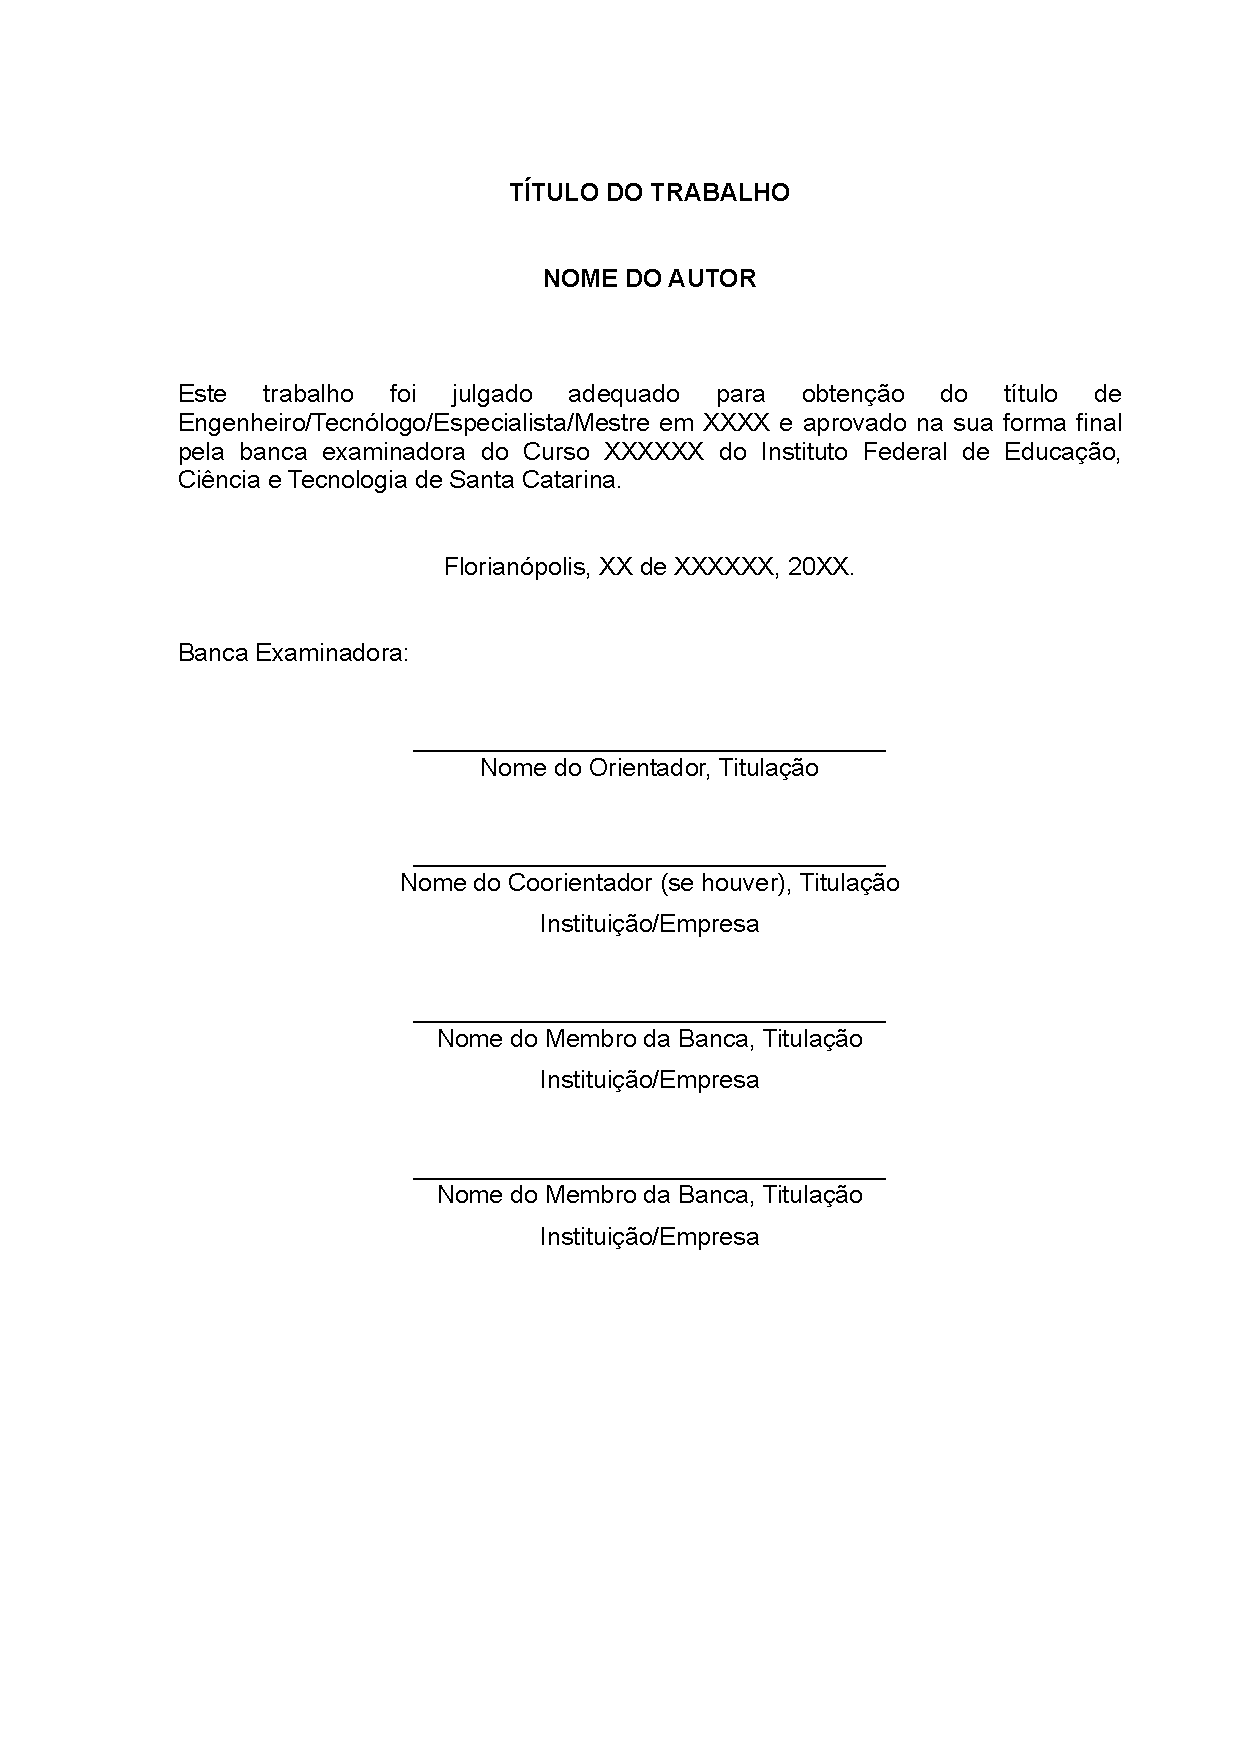
\includepdf[pages=-]{pdf/tcc-aprovado.pdf}

%\cleardoublepage

%---------------------------------------------------------------------%
% Dedicatória
%---------------------------------------------------------------------%
\begin{dedicatoria}
    \vspace*{\fill}
	\begin{flushright}

\fcolorbox{red}{red}{|||||||||||||||||||||||||||||||||}\\
\fcolorbox{red}{red}{|||||||||||||||||||||||||||||||||}\\
\fcolorbox{red}{red}{|||||||||||||||||||||||||||||||||}\\
\fcolorbox{red}{red}{|||||||||||||||||||||||||||||||||}\\
\fcolorbox{red}{red}{|||||||||| AO AVANÇO}\\
\fcolorbox{red}{red}{  E PERSISTÊNCIA}\\
\fcolorbox{red}{red}{||||||||| DA CIÊNCIA,}\\
\fcolorbox{red}{red}{PRINCIPALMENTE}\\
\fcolorbox{red}{red}{|||||||||||||||||||||||| NOS}\\
\fcolorbox{red}{red}{|||||||||||| PERÍODOS}\\
\fcolorbox{red}{red}{ CONTURBADOS. }\\
\fcolorbox{red}{red}{|||||||||||||||||||||||||||||||||}\\
\fcolorbox{red}{red}{|||||||||||||||||||||||||||||||||}\\
\fcolorbox{red}{red}{||||||||||||||| A TODOS}\\
\fcolorbox{red}{red}{|||||||||| QUE A VIDA}\\
\fcolorbox{red}{red}{||||||||||||| CESSOU...}\\
\vspace{1.15cm}

\fcolorbox{red}{red}{|||||||| ...POR FALSA}\\
\fcolorbox{red}{red}{|||||| INFORMAÇÃO,}\\
\fcolorbox{red}{red}{DESINFORMAÇÃO}\\
\fcolorbox{red}{red}{||||||| OU NEGAÇÃO}\\
\fcolorbox{red}{red}{||||||||||| DA MESMA.}
      
	\end{flushright}
\end{dedicatoria}




%---------------------------------------------------------------------%
% Agradecimentos
%---------------------------------------------------------------------%
\begin{agradecimentos}
    Elemento opcional que não pode ultrapassar o limite de uma página.
\end{agradecimentos}
% ---

%---------------------------------------------------------------------%
% Epígrafe
%---------------------------------------------------------------------%
\begin{epigrafe}
    \vspace*{\fill}
	\begin{flushright}
        		"If I have seen further, it is by standing on the shoulders of giants"\\(Sir Isaac Newton).
	\end{flushright}
\end{epigrafe}

%---------------------------------------------------------------------%
% RESUMOS
%---------------------------------------------------------------------%
% resumo em português
\setlength{\absparsep}{18pt} % ajusta o espaçamento dos parágrafos do resumo
\renewcommand{\baselinestretch}{1} 
\begin{resumo}
    % O resumo deve mostrar a natureza e o objetivo do trabalho, o método que foi empregado, os resultados e as conclusões. O resumo deve conter entre 150 e 500 palavras e constitui-se de um único parágrafo, sem recuo.
A dengue é uma doença viral infecciosa, transmitida pela picada da fêmea do mosquito \latim{Aedes aegypti} (Linnaeus, 1762). Atualmente é um dos principais problemas de saúde coletiva no mundo. Está presente nas regiões tropicais e subtropicais do planeta, sendo estimado que 390 milhões de pessoas sejam infectadas anualmente pelos quatro sorotipos. Há tendência de resposta à sazonalidade em relação ao número de focos de dengue, na qual os meses com temperaturas mais elevadas se observa crescimento, principalmente quando retroagidos por um período de 30 dias; e tem diminuição nos meses mais frios, logo, temperatura é um elemento crítico para o desenvolvimento do mosquito. A geomedicina porporciona base para o próprio estudo espacializado de doenças, sendo assim, a seguinte proposta tem o objetivo direto de observar a relação entre o histórico e a distribuição de focos do vetor biológico \latim{Aedes aegypti}, transmissor das principais arboviroses no Estado de Santa Catarina (dengue, febre amarela, zika e chikungunya), e o comportamento de elementos climáticos. Foram utilizados dados de temperatura do \ingles{\acrfull{GFS}}, após isso, foi sintetizado o \acrfull{ICOb}, utilizando-se o \acrfull{LACOb}. Dessa forma, pode-se modelar e visualizar cartograficamente esses resultados, como previsão de aumento regionalizado de focos de \latim{Aedes aegypti} no Estado de Santa Catarina. Ademais, pretende-se alcançar outros objetivos, tais como: mapeamento das ocorrências dentro do Estado, análise de dados entomológicos e epidemiológico; além de relacionar aos dados socioeconômicos da população catarinense. Investigar esses múltiplos aspectos e compreender essas informações auxiliam no processo de tomada de decisões, buscando, assim, uma melhor resposta frente a zoonoses emergentes e re-emergentes.
 
   \noindent 
    \textbf{Palavras-chave}: Variabilidade Climática. Geomedicina. Saúde Única. Zoonose. 
\end{resumo}

% resumo em inglês
\renewcommand{\baselinestretch}{1} 
\begin{resumo}[Abstract]
 \begin{otherlanguage*}{english}
   % The abstract should show the nature and scope of work, the method that was used, the results and conclusions. The abstract may contain between 150 and 500 words, and it must be only one paragraph. 
 Dengue is an viral infectious disease transmitted by the female mosquito \latim{Aedes aegypti} (Linnaeus, 1762). Nowadays, it is one of the main public health problems in the world. It is present in the tropical and subtropical regions of the planet, with an estimated 390 million people are infected annually with all four serotypes. There is a tendency to respond to seasonality in relation to the number of dengue outbreaks, in which the months with higher temperatures are observed growth, mainly when retroacted for a period of 30 days; and observe decrease in the colder months, therefore, temperature is a critical element for the growth of the mosquito. Geomedicine provides a basis for the spatialized study of diseases, thus, this project has the direct objective of observing the relationship between the history and the distribution of outbreaks of the biological vector \latim{Aedes aegypti}, transmitter of the main arboviruses in the State of Santa Catarina (dengue, yellow fever, zika and chikungunya), and the observation of climate elements. The temperature data were used from the \acrfull{GFS}, after which the Combined Index by Observation [\acrfull{ICOb}] was synthesized, using the Observed High Correlation Limit [\acrfull{LACOb}]. In this way, it is possible to model and visualize these results cartographically, as forecast of a regionalized increase in outbreaks of \latim{Aedes aegypti} in the State of Santa Catarina. Furthermore, it is intended to achieve other objectives, such as: mapping of occurrences within the State, analysis of entomological and epidemiological data; in addition to relating to socioeconomic data of the Santa Catarina population. Investigate these multiple aspects and understand this information assist in the decision-making process, thus seeking a better response to emerging and reemerging  zoonotic diseases. 

   %\vspace{-0.8cm}
 
   \noindent 
   \textbf{Keywords}: Climate Variability. Geomedicine. One Health. Zoonosis.  
 \end{otherlanguage*}
\end{resumo}


%---------------------------------------------------------------------%
% inserir lista de ilustrações
%---------------------------------------------------------------------%
\renewcommand{\listfigurename}{Lista de Figuras}
\pdfbookmark[0]{\listfigurename}{lof}
\listoffigures*
\cleardoublepage

%---------------------------------------------------------------------%
% inserir lista de quadros
%---------------------------------------------------------------------%

\renewcommand{\listquadroname}{Lista de quadros}
\newfloat{quadro}{\quadroname}{loq}[chapter]
\setfloatlocations{quadro}{hbtp}
\newlistof{listofquadros}{loq}{\listquadroname}
\newlistentry{quadro}{loq}{0}
\renewcommand{\cftquadroname}{\quadroname\space}
\renewcommand*{\cftquadroaftersnum}{\hfill\textendash\hfill}
\counterwithout{quadro}{chapter}
\listofquadros* 
\cleardoublepage



%---------------------------------------------------------------------%
% inserir lista de tabelas
%---------------------------------------------------------------------%
\pdfbookmark[0]{\listtablename}{lot}
\listoftables*
\cleardoublepage

%---------------------------------------------------------------------%
% inserir lista de listings
%---------------------------------------------------------------------%
%\pdfbookmark[0]{\lstlistlistingname}{lol}
%\listoflistings
%\cleardoublepage

%---------------------------------------------------------------------%
% inserir lista de abreviaturas e simbolos
%---------------------------------------------------------------------%
%\listofabrev{tex/00-Abreviaturas}
% \imprimirlistadeabreviaturas
%ESTOU USANDO \usepackage{glossaries}---------------------------------%
\printglossary[title = Lista de Abreviaturas e Siglas, type = \acronymtype]
%---------------------------------------------------------------------%

% \imprimirlistadesimbolos
\cleardoublepage

%---------------------------------------------------------------------%
% inserir o sumario

%---------------------------------------------------------------------%


\setlength{\cftbeforechapterskip}{4pt plus 0pt}
\pdfbookmark[0]{\contentsname}{toc}
\tableofcontents*
\cleardoublepage

% ----------------------------------------------------------
% ELEMENTOS TEXTUAIS
% ----------------------------------------------------------
\textual
\pagestyle{parpage}%
\aliaspagestyle{chapter}{parpage}
% ----------------------------------------------------------
% Inclusão dos capítulos que estão em outros arquivos .tex
% ----------------------------------------------------------

\chapter{Introdução}
%Máximo 2pg:

% Contextualizar o Clima de SC;
\indent O clima é a composição do tempo meterológico ao longo de um período, pelo menos trinta anos, em um determinado território. (\acrlong{SC}, \citeyear{AtlasSCnatureza}, pg-75).

\indent O estado de \acrfull{SC} está localizado no sul do Brasil, região onde ocorrem totais pluviométricos elevados e precipitação bem distribuída ao longo do ano. Parte desse comportamento é devido a atuação sistemas meteorológicos como: \acrfull{FF}, Sistemas Frontais, Clicones Extratropicais, Vórtices Clicônicos em Altos Níveis, Bloqueios Atmosféricos e \acrfull{CCM}, além a influência indireta da \acrfull{ZCAS} \cite{reboita2010}.

\begin{center}
\textcolor{red}{Incluir \cite{Guerra2023Regionalizacao}}
\end{center}

\textcolor{red}{CONTEXTUALIZAR TEMPERATURA/CLIMA EM SC}

\textcolor{red}{CONSIDERAÇÕES AQUI!}

%Contextualizar Dengue;
\indent Assim, sendo expresso no Guia de Vigilância em Saúde, o mosquito \latim{Aedes aegypti} pode comumente transmitir algumas arboviroses, como: Dengue, Zika e Chikungunya \cite{GuiaVigSaúde22}; o \latim{A. aegypti} também é responsável pela transmissão de Febre Amarela em ciclo urbano. Ainda informado pelo \citeonline{GuiaVigSaúde22}, a dengue possui como agente etiológico o \acrfull{DENV}, sendo agrupado em quatro sorotipos distintos (\acrshort{DENV}-1, \acrshort{DENV}-2, \acrshort{DENV}-3 e \acrshort{DENV}-4), e é uma das zoonoses vetorizadas por artrópodes mais relevantes nas Américas.

\textcolor{red}{Relacionar Clima e Dengue (Geral)}

\indent Em estudo realizado por \citeonline{Drumond2020Dinamica}, entre 2007 e 2017 no \acrfull{DF}, o número de casos foi maior nos primeiros semestres, particularmente entre o final do verão e o início do outono. Este período  coincide com o final do período chuvoso. Os autores também observaram que a dengue se manteve hiperendêmica no \acrlong{DF}, tendo casos registrados durante todos os meses do ano e circulação dos quatro sorotipos do vírus.

\begin{center}
\textcolor{red}{CONSIDERAÇÕES AQUI!}
\end{center}

\textcolor{red}{INCLUIR OUTROS ESTUDOS}

\textcolor{red}{Relacionar Clima e Dengue (SC)}

\textcolor{red}{INCLUIR OUTROS ESTUDOS}

\textcolor{red}{Relacionar Clima e Dengue (SC)}

{\color{red} \rule{\linewidth}{0.5mm}}

\color{red} INÍCIO DE BLOCO DE CONSIDERAÇÃO

\indent O Estado catarinense apresentou em 2014 apenas três casos autóctones de dengue (infectados dentro do próprio estado), no município de Itajaí, e 66 casos importados. Naquele mesmo período, a região serrana e planalto não apresentavam focos \cite{Matiola2020Dissertação}. De acordo com a \citeonline{Informe5DiveSE9/23}, para este momento (final de março de 2023 - décima segunda semana epidemiológica), há focos de dengue distribuídos por todas as regiões catarinenses.

FINAL DE BLOCO DE CONSIDERAÇÃO

{\color{red} \rule{\linewidth}{0.5mm}}

\color{black}

\indent Segundo \citeonline{Matiola2020Dissertação}, em \acrlong{SC}, há tendência de resposta à sazonalidade nos meses com temperaturas mais elevadas, observando-se o crescimento do número de focos do \latim{Aedes} sp.,  principalmente quando retroagidos por um período de 30 dias, além da diminuição nos meses mais frios.

\indent Portanto, a temperatura é um fator crítico para o desenvolvimento do mosquito no estado catarinense. com relação a previsibilidade das ocorrências, \citeonline{Matiola2020Dissertação} também sugerem que a precipitação do mês que antecede o registro do foco influencia no desenvolvimento do mosquito, corroborando com correlações maiores quando retroativas.

\begin{center}
\textcolor{red}{CONSIDERAÇÕES AQUI!}
\end{center}
\textcolor{red}{INCLUIR INFODENGUE COMO MODELO PREDITIVO}

\textcolor{red}{Contextualizar estudos com modelos Dengue/A.a}

\textcolor{red}{INCLUIR OUTROS ESTUDOS}

\textcolor{red}{Citar \latim{Aedes albopictus}}

\indent Por simplificação, o projeto tratará ambos os pernilongos \latim{Aedes aegypti} (Linnaeus, 1762) e \latim{Aedes albopictus} (Skuse, 1895) apenas como gênero \latim{Aedes} sp. (Meigen, 1818), da família \latim{Culicidae} (Meigen, 1818). Nomenclatura científica seguindo taxonomia citada e arquivada pelo Museu Nacional de História Natural, Instituto Smithsonian (\citeyear{ITIS}), através do Sistema Integrado de Informação Taxonômica (\acrfull{ITIS}).

%%%%%%%%%%%%%%%%%%%%%%%%%%%%%%%%%%%%%%%%%%%%%%%%%%%%%%%%%%%%%%%%%%%%%%%%%%%%
\newpage
\section{Justificativa}
%1parágrafo
\indent Pelo exposto, a dengue é uma zoonose emergente no estado de \acrlong{SC} e se faz necessário relacionar a nova dinâmica climatológica aos comportamentos de distribuição de \latim{Aedes} sp. e ocorrência de dengue.

\begin{center}
\textcolor{red}{CONSIDERAÇÕES AQUI!}
\end{center}
\textcolor{red}{Necessidade de reconhecer relação das variáveis climáticas com a reprodução do mosquito, mudança no cenário da doença no estado associado a disseminação do mosquito...}

\indent DESCRITIVO > PREDITIVO > PRESCRITIVO
 
%%%%%%%%%%%%%%%%%%%%%%%%%%%%%%%%%%%%%%%%%%%%%%%%%%%%%%%%%%%%%%%%%%%%%%%%%%%%%
 \section{Objetivo Geral}
 Avaliar a relação entre os focos de \latim{Aedes} sp. e os casos de dengue e a condição climatológica predominante sobre o Estado de \acrlong{SC}, visando elaborar um modelo preditivo de proliferação do vetor biológico e da doença.

\begin{center}
\textcolor{red}{CONSIDERAÇÕES AQUI!}\\ 
\end{center}

 % Elaborar um modelo preditivo para a proliferação do mosquito \latim{Aedes aegypti}, a partir de análise das condições meteorológicas do Estado de \acrlong{SC}.

 % Analisar a relação entre a reprodução do mosquito \latim{Aedes aegypti} e as condições meteorológicas no Estado de \acrlong{SC}.

 
\section{Objetivos Específicos}
As estratégias para atingir o objetivo geral são descritas como objetivos específicos abaixo:

\begin{alineas}
\item Analisar estatisticamente padrões das séries temporais, a partir das regiões climatológicas determinadas por \citeonline{Guerra2023Regionalizacao}, para modelagens futuras; \textcolor{red}{REFINAR!}
\item Elaborar modelo preditivo para a proliferação dos mosquitos do gênero \latim{Aedes} sp. e os casos confirmados de dengue, a partir de análise das condições meteorológicas do Estado de \acrlong{SC}.
\item Analisar estatisticamente as modelagens para validação das ferramentas;
\item Realizar um estudo de caso para melhor entender o fenômeno a partir de um ciclo anual;
\item Sintetizar o \acrfull{PTT}:
\subitem Sistema Computacional;
\subitem Visualização Cartográfica desses resultados.
    %Último deve relacionar o produto
\end{alineas}
 % Introdução + Justificativa + Objetivos
\chapter{Fundamentação Teórica}

Esta seção apresenta uma breve contextualização sobre questões sanitárias e climatológicas. Foi elaborada através de  fichamento do material científico acessado: livros, artigos, \ingles{sites}, boletins e informes oficiais, dentre outros. Essa revisão bibliográfica servirá como base para conciliar diferentes áreas do conhecimento, assim como facilitar o entendimento de terminologias abordadas no presente estudo.

\section{Caracterização do Clima e Ambiente}

\subsection{Climatologia e Sistemas Meteorológicos de Santa Catarina (SC)}

\indent "Clima é a sucessão habitual dos diversos tipos de tempo que compõem o cenário atmosférico de uma região ao longo de um período de pelo menos trinta anos" (\acrlong{SC}, \citeyear{AtlasSCnatureza}, pg-75 ).

\indent Segundo \citeonline{reboita2010}, \acrlong{SC} se encontra no setor R4 de precipitação, sendo similar ao restante do sul do Brasil, ao Paraguai e ao Uruguai. No entanto, utilizando a classificação de \citeonline{MERGEatual}, o Estado catarinense está compreendido no setor R1 de precipitação. Ambos os autores defendem um total pluviométrico elevado e bem distribuído ao longo do ano. Esse comportamento se deve a atuação de sistemas meteorológicos na região. A presença de vórtices ciclônicos e cavados em altos níveis sobre a costa oeste da América do Sul favorece o desenvolvimento de ciclones e \acrlong{FF} nesses setores (R1 \cite{MERGEatual} e R4 \cite{reboita2010}). Dessa forma, condições ciclogenéticas e frontogenéticas se desenvolvem sobre \acrlong{SC}.

\indent Os sistemas frontais, que se deslocam do sul em sentido Noroeste-Nordeste, passando pela Argentina e adentrando o Brasil, causam precipitação atuando diretamente na região ou fornecendo condições para o desenvolvimento de \acrfull{LI} pré-frontais \cite{reboita2010}.

\indent As condições favoráveis à ocorrência de tempestades aumentam quando o processo convectivo é acoplado a um ou mais sistemas de instabilidade, como vórtices ciclônicos, baixas térmicas, \acrfull{JBN} ou a passagem de \acrlong{FF} pelo litoral sul do Brasil (\acrlong{SC}, \citeyear{AtlasSCnatureza}).

DESCREVER \acrlong{CCM};

DESCREVER Sistema Clicônico em Médios Níveis (vírgula invertida);

DESCREVER \acrlong{ZCAS};

DESCREVER  sistemas de circulação locais (brisas).

\indent De acordo com o Atlas Geográfico de \acrlong{SC} (\citeyear{AtlasSCnatureza}), os maiores índices de precipitação anuais são observados na região Oeste, Grande Florianópolis e Litoral Norte. Entretanto, no Litoral Sul, entre Araranguá e Laguna, os totais anuais desses índices são os menores. O efeito sazonal da dinâmica dos sistemas atmosféricos, sobretudo pelas altas pressões, e a influência da orografia, principalmente por planícies e planaltos, resultam em variações na distribuição espacial de elementos climáticos, como temperatura e precipitação, que se observa menores temperaturas médias em regiões de maiores altitudes e tendência com maiores acumulados de precipitação próximos às serras. Em consonância com \citeonline{Oliveira2022Sistema}, a definição do sistema de anticiclone é tida como centros de alta pressão atmosférica.

\begin{citacao}
"...A maior influência ocorre pelo anticiclone Migratório Polar, centro de ação da Massa de Ar Polar, úmida quando a trajetória é marítima (mPa) e seca quando a trajetória é continental, sempre fria (mPc); pelo anticiclone do Atlântico, centro de ação da Massa Tropical Atlântica (mTa), quente e úmida e pela depressão do Chaco, que é o centro de ação da Massa Tropical Continental (mTc), quente e seca (\acrlong{SC}, \citeyear{AtlasSCnatureza}, pg-77)." 
\end{citacao}

\indent "Os elementos que constituem as condições momentâneas de tempo passam a ser denominados elementos climáticos quando utilizados para fins de estudos relacionados ao clima" (\acrlong{SC}, \citeyear{AtlasSCnatureza}, pg-75).

\subsection{Aspectos Bióticos e Abióticos}

\indent Cabe destacar que, antes da promulgação da Constituição Federal de 1988, o Estado brasileiro estabelece a \acrfull{PNMA}, que tem a preservação, melhoria e recuperação da qualidade ambiental proprícia à vida como objetivo principal, conforme a luz da lei. Essa mesma política define recursos ambientais, englobando fauna, flora, elementos da biosfera, solo, subsolo, mar territorial, águas interiores, estuários, águas subterrâneas, águas superficiais e atmosfera, além de definir meio ambiente como "o conjunto de condições, leis, influências e interações de ordem física, química e biológica, que permite, abriga e rege a vida em todas as suas formas" \cite{BRASIL1981LeiPNMA}. Logo, meio ambiente é um conceito amplo que, dependendo da doutrina, vai além dos aspectos naturais.  

\indent O Estado catarinense está situado no sul do Brasil, tendo limites com o Estado do Paraná ao norte e, ao sul, com o Estado do Rio Grande do Sul. Esses três Estados  formam a região Sul do Brasil. \acrlong{SC} também tem limites a leste com o oceano Atlântico e a oeste com a República Argentina.  O Estado ocupa aproximadamente 1\% da território nacional e  cerca de 16\% da área total da Região Sul (\acrlong{SC}, \citeyear{AtlasSCterritorio}).

\indent É possível notar diferentes paisagens em \acrlong{SC}; essas, criadas por formas de relevos variadas. Sob esses aspectos, pode-se observar os principais compartimentos de relevo no Estado catarinense: Planície (Costeira), Serras (do Mar, do Tabuleiro-Itajaí e Geral), Planaltos (de São Bento do Sul, de Lages, dos Campos Gerais e Dissecado Rio Iguaçu-Rio Uruguai), Patamares (de Mafra, do Alto Rio Itajaí e da Serra Geral) e Depressão (da Zona Carbonífera) (\acrlong{SC}, \citeyear{AtlasSCnatureza}).

\indent O relevo define a grande divisão regional de \acrlong{SC}: região do
litoral e encostas, e região do planalto. Somado a esse relevo singular, o clima explica o processo colonial tardio do Estado catarinense (\acrlong{SC}, \citeyear{AtlasSCpopulacao}).

\indent Como verificado no Atlas Geográfico de \acrlong{SC} (\citeyear{AtlasSCnatureza}), hipsometria do Estado catarinense é muito diversa, variando de mais de 1.800 metros ao zero, no nível do mar. Esse comportamento ocorreu pelo soerguimento epirogenético durante o período Terciário, que afetou toda a porção leste do continente Sul Americano, também por conta de processos erosivos e a diferentes resistências de rochas. A zona costeira de \acrlong{SC} varia de 0 a 200 metros, atingindo 400 metros em regiões próximas ao litoral, no baixo curso do rio Itajaí-Açú e no fundo do vale do rio Uruguai e seus afluentes. A maior parte da bacia hidrográfica do Itajaí se encontra entre 400 e 800 metros, assim como parte do vale do rio Uruguai e regiões do Meio Oeste catarinense. Altitudes entre 800 e 1.200 metros são mais comuns em \acrlong{SC}, sendo decorrentes de serras, escarpas, planaltos e patamares. Nessas altitudes se encontram os divisores de água do Estado catarinense. "Por causa destas altitudes, as temperaturas são mais amenas e o clima se torna mais propício para o cultivo de frutas de clima temperado" (\acrlong{SC}, \citeyear{AtlasSCnatureza}). "Altitudes maiores do que 1.200 m são pouco comuns em Santa Catarina, [...] as elevadas altitudes permitem, em condições meteorológicas favoráveis, a ocorrência de neve..." (\acrlong{SC}, \citeyear{AtlasSCnatureza}).

\indent  O Atlas Geográfico de \acrlong{SC} (\citeyear{AtlasSCnatureza}) também comenta que remanescentes de cobertura primária ainda são existentes, porém são pequenos grupamentos e estão em locais de difícil acesso. Parte dessa fragmentação, também em coberturas secundárias, ocorre devido ao avanço agropecuário em \acrlong{SC} e o  processo de urbanização, principalmente, na segunda metade do século XX. A cobertura vegetal catarinense é biodiversa, resultante de variedades de climas, relevo e solos. A vegetação litorânea é composta por restinga e mangue. As coberturas florestais ocorrem nas encostas de serras e vales de vertente atlântica (floresta ombrófila densa), nos planaltos (floresta ombrófila mista) e vales do rio Uruguai e afluentes (floresta estacional decidual subtropical). Em elevadas altitudes, acima de 1.500 mestros, a cobertura vegetal é composta por floresta nebular e campos de altitude. Também ocorre vegetação campestre numa altitude aproximada de 800 metros, tendo precipitação bem distribuída ao longo do ano e médias de temperatura inferiores a 15 C. "Um tipo de floresta muito típico são os Faxinais, que aparecem em altitudes entre 700 e 1.200 metros [...] são associações mistas de espécies da mata Pluvial com elementos da floresta de Araucária" (\acrlong{SC}, \citeyear{AtlasSCnatureza}).

\subsection{População Catarinense e Contexto Histórico}

\indent Como \citeonline{Lages2004Territorios} argumentam, "território é o espaço apropriado por um ator, sendo definido e delimitado por e a partir de relações de poder, em suas múltiplas dimensões". Os próprios autores ainda definem a noção de espaço, que representa uma abstração maior, tendo o território como produto da intervenção e do trabalho dos atores sobre determinado espaço. "Tal como a cultura, o território não é rígido, mas produto da dinâmica histórica das sociedades" (\acrlong{SC}, \citeyear{AtlasSCpopulacao}).

\indent Como ressaltado no Atlas Geográfico de \acrlong{SC} (\citeyear{AtlasSCpopulacao}) o território era ocupado por povos originários há milhares de anos, muito antes da colonização. São conhecidos três grupos indígenas, denominados: Guarani, Kaingang e Xokleng. "Os Xokleng no Alto Vale do Itajaí voltaram a se definir Laklãnõ recentemente". Com o processo histórico de colonização, houve redução  territorial desses povos, principalmente por uma política indigenista de aldeamento.

\indent O grupo Guarani possuia uma agricultura mais sofisticada e ocupava terras baixas, principalmente do litoral sul brasileiro e várzeas da bacia do rio da Prata. "Há mais de um milênio foi iniciada a ocupação Guarani na costa Atlântica sul, inclusive de Santa Catarina, cujas datações mais antigas estão entre os anos 930 e 980 em Imbituba". Os Laklãnõ (Xokleng) se deslocavam no território entre mata Atlântica e florestas de araucárias do planalto. Os Kaingang tinham as terras altas como território, isso por associação à mitologia do grande dilúvio e por predomínio da mata de araucária, do qual proporcionava a base alimentar (\acrlong{SC}, \citeyear{AtlasSCpopulacao}).

\begin{citacao}
"Os indígenas resistiram a esse processo de esbulho do seu patrimônio e de violência
física. O conceito de resistência deve ser amplo, não no sentido de luta armada, mas
de estratégias cotidianas de enfrentamento aos ditames da política indigenista. [...] Atualmente, é importante salientar que os povos indígenas habitantes do Brasil, incluindo os povos que vivem em \acrlong{SC}a, estão em crescimento demográfico, sendo uma característica desse processo o reconhecimento da sua própria identidade" (\acrlong{SC}, \citeyear{AtlasSCpopulacao}, pg-47).
\end{citacao}

\indent Assim descrito por \acrlong{SC} (\citeyear{AtlasSCpopulacao}), os estados da região sul brasileira, assim como o território catarinense, foram conquistados e colonizados de forma tardia, a partir do século XVII. "Certamente dentre os elementos referentes ao quadro natural, o clima é o mais ressaltado como um dos determinantes na estruturação tardia da formação meridional brasileira" (\acrlong{SC}, \citeyear{AtlasSCpopulacao}). Seria muito difícil, para o universo colonial marcado pela tropicalidade, oferecer aos interesses comerciais da Metrópole Portuguesa uma produção que atendesse, abaixo do Trópico de Capricórnio, ao predomínio do clima subtropical.

\indent Nesse mesmo século, XVII, fazia-se necessário um sistema defensivo litorâneo da ilha de \acrlong{SC}. Porém, a partir do século XVIII, houve a incorporação do litoral catarinense ao sistema econômico colonial português, o que levou a migração de açorianos e madeirenses para o território. Também iniciando nesse período, surgiram novos povoados na estrada das tropas para pouso e descanso, sendo anexados ao território catarinense no século XIX (\acrlong{SC}, \citeyear{AtlasSCterritorio}). "... A exploração das terras do planalto começa com os paulistas no século XVIII, instalando a pecuária extensiva nas manchas de campos naturais de Lages, Curitibanos e Campos Novos" (\acrlong{SC}, \citeyear{AtlasSCpopulacao}).

\begin{citacao}
"Santa Catarina vivencia seu processo de conquista e colonização, tardio em cerca
de cem anos frente ao Nordeste e Sudeste brasileiros, com povos fruto do crescimento demográfico da Colônia, caracterizando um processo migratório interno, no sentido norte-sul. Isto tanto no século XVII (Litoral), quanto ainda no XVIII (Planalto), mesmo século em que também se inicia a migração externa com populações vindas de além-mar, no caso da 2ª ocupação do litoral catarinense. A partir do século XIX tal processo imigratório se intensifica com a ocupação dos vales atlânticos e encostas pelos imigrantes europeus, excedente populacional  relativo a uma Europa em transformação frente ao avanço e desenvolvimento do modo de produção capitalista" (\acrlong{SC}, \citeyear{AtlasSCpopulacao}, pg-22). 
\end{citacao}

\indent Por meados do século XIX, algumas regiões européias, já em fase industrial, atravessam um período de crise econômica e turbulência política. Esse cenário de crise foi provocado pela expansão do capitalismo, o que levou ao aprofundamento e ampliação do processo de expropriação, responsável pelo próprio crescimento demográfico europeu. É nesse contexto que as transformações em áreas de capitalismo
tardio levam milhões de emigrantes a cruzar o oceano em busca de novas oportunidades. "...Foram criados, principalmente por alemães e italianos, vários núcleos rurais e urbanos em áreas correspondentes aos vales atlânticos e encostas dos rios Itajaí, Cachoeira, Cubatão, Tijucas, Tubarão, Urussanga e Araranguá" (\acrlong{SC}, \citeyear{AtlasSCpopulacao}).

\indent Também pela metade do século XIX, o Governo Imperial criou mais uma colônia militar, a do Chapecó. "Implantada em 1882 em área correspondente hoje ao município de Xanxerê". Além de fazer a guarda da fronteira, também protegia a porção mais a oeste do caminho das tropas, como as primeiras colônias nas encostas do planalto a leste. No início do século XX, instalaram-se pequenas propriedades rurais policultoras (Joaçaba, Chapecó e Concórdia), por conta da expansão demográfica do Rio Grande do Sul, principalmente com a chegada da ferrovia São Paulo-Rio Grande do Sul (1908-1910), no vale do rio do Peixe (\acrlong{SC}, \citeyear{AtlasSCpopulacao}).

\indent Também devemos tomar nota da população de origem africana que, assim como os povos indígenas, foi escravizada durante os períodos colonial e imperial. "Das origens, na África, houve predomínio da região Centro-Ocidental (Congo, Angola, Benguela), com alguma presença de africanos orientais (Moçambique) e ocidentais (Mina, Jejes)". Há registros que apontam para o crescimento gradual de africanos escravizados e indígenas administrados, desde o século XVII, com a fundação de São Francisco do Sul, Desterro e Laguna. Ainda assim, a captura e a escravização de indígenas estava condenada por parte das autoridades judiciais da capitania de São Paulo na década de 1720. Fato esse que intensificou o tráfico transatlântico de escravos africanos para os territórios portugueses na América nos séculos XVIII e XIX, marcando o início de uma virada demográfica. Parte desses afrodescendentes foi utilizada como mão-de-obra para contrução de fortificações no litoral, estações baleeiras, trabalho em engenhos de farinha de mandioca, açúcar, aguardente e na lida com o gado no planalto (\acrlong{SC}, \citeyear{AtlasSCpopulacao}). 

\begin{citacao}
"Desde o século XIX, a autoimagem de Santa Catarina é a de uma província ou um estado europeu, uma singularidade que nos distanciaria do restante do Brasil, marcado pela mestiçagem. A associação de “branco” com “europeu”, e deste com “civilização” e “progresso”, é um traço persistente do senso comum. Embora seja
inegável tanto a presença quanto a participação de descendentes de europeus na
constituição demográfica e econômica de Santa Catarina, o efeito colateral é a invisibilização da população de origem africana" (\acrlong{SC}, \citeyear{AtlasSCpopulacao}, pg-79).
\end{citacao}

\indent Não coincidentemente, o Brasil tem registro de dengue desde o século XIX, relatado em literatura por epidemias no Rio de Janeiro (1846) e em São Paulo (1852) \cite{Valle2015Dengue}.

\section{Contextualização sobre Saúde}

\subsection{Saúde para Ciências Exatas e da Terra}

\begin{center}
\textcolor{red}{CONSIDERAÇÕES AQUI!}\\
\textcolor{red}{JOÃO: Geomedicina (Geografia médica, Geografia da saúde, medicina social, espaço).}\\
\end{center}

\indent Sendo o \acrfull{PCAM} vinculado a Ciências Exatas e da Terra, particularmente dentro das GeoCiências, de acordo com sistematização das áreas de conhecimento da \acrfull{CAPES} (\citeyear{CAPES_Tabela_Conhecimento}) e publicizado pelo \acrfull{CNPq} \citeyear{CNPq_Tabela_Conhecimento}), deve-se atentar para nomenclaturas e abordagens sobre saúde.

\indent Segundo \citeonline{Geomedicine2012Davenhall}, a Geomedicina é definida como uma nova área de inteligência médica que utiliza dados e infraestrutura espaciais para benefício da prória saúde humana; para \citeonline{Geomedicine1990JulLag}, é uma área da ciência que observa influências e relações do meio ambiente com a distribuição espacial de agravos em saúde de homens e animais.

\indent DESCREVER Geografia médica.

\indent DESCREVER Geografia da saúde.

\indent Medicina social/espaço. RENE AREIA, Associação de Medicina Social da Bélgica "enfatizou a importância do social, político e cultural na origem e persistência de doenças epidêmicas".

\begin{center}
\textcolor{red}{CONSIDERAÇÕES AQUI!}\\
\indent \textcolor{red}{JOÃO: Tópico para Saúde Coletiva/Pública e Saúde Única\\(SEPARAR EM TÓPICOS DISTINTOS)}\\
\end{center}

%\subsection{Saúde: Coletiva e Única}

\subsection{Saúde Coletiva}

\indent Durante a antiguidade grega, precisamente no século V a.C., Hipócrates defendia a idéia de que um ambiente saudável estava ligado com a própria saúde do população. Ele é considerado o pai da Medicina e adotava a visão de Saúde Pública integrada ao ambiente \cite{CFMVSaude}.

\indent Foucault - Medicina Social: Medicina de Estado; Medicina Urbana e Medicina da Força de Trabalho. 

\indent Salubridade x Insalubridade

\indent Adotando o conceito de saúde da Carta Magna para Saúde Mundial, desde planejamento de criação até a execução atual da \acrfull{OMS}, tem-se saúde como um estado de completo bem-estar físico, mental e social, e não apenas como a ausência de doença ou enfermidade \cite{OMS2024S1, ParranHEALTH}.

\indent BRASIL. Lei nº 8.080, de 19 de setembro de 1990. Lei Orgânica da Saúde. Dispõe sobre as condições  para a promoção, proteção  e  recuperação  da  saúde,  a  organização  e  o  funcionamento  dos  serviços correspondentes  e  dá  outras providências.
% https://www.planalto.gov.br/ccivil_03/leis/l8080.htm


\indent Abordagens articuladas à saúde: Foucault, Butler e Laqueur

\indent Maria Cecília Minayo (2001), reforma sanitária.

\indent Convergências epistemológicas entre a Bioética e saúde coletiva discutidas por Junges
e Zoboli (2012)

\indent Segundo Marsiglia (2013) o uso do termo “coletivo” no campo da saúde coletiva é de
fundamental importância, haja vista que
% https://www.teses.usp.br/teses/disponiveis/5/5137/tde-09082017-100757/publico/MarceloJosedeSouzaeSilva.pdf


\subsection{Saúde Única}

\indent Em 1968, a \acrfull{OPAS} convoca a \acrfull{RIMSA}, realizando proteção e promoção da saúde humana e animal por meio da cooperação técnica em saúde pública veterinária, além de manter enfoque multissetorial \cite{S1_OPAS_OMS}. O termo Medicina Única foi concebido pelo médico-veterinário Calvin W. Schwabe (1927-2006) em sua obra "\ingles{Veterinary Medicine and Human Health}” em 1984, reforçando a importância da junção entre saúde humana, animal e ambiental \cite{CFMVSaude}. Aos poucos, o mundo foi despertando para a importância da interação entre saúde e meio ambiente.

\indent Durante a Conferência das Nações Unidas sobre Meio Ambiente e Desenvolvimento no Rio de Janeiro em 1992, conhecida como EcoRio92, discutiram-se as bases para avançar esforços conjugados quanto à colaboração entre setores de saúde e meio ambiente. Logo, em 1995, foi adotada a Carta Pan-Americana sobre Saúde e Meio Ambiente no Desenvolvimento Humano Sustentável \cite{S1_OPAS_OMS}, porém a evolução do termo para Saúde Única ocorreu no século XXI \cite{CFMVSaude}. 

\indent No ano de 2004, em Nova Iorque, especialistas se reuniram para debater e propor ações em resposta à potencial dinâmica de doenças entre humanos, animais domésticos e fauna silvestre. Naquela época, principalmente, alertar sobre ebola, influenza aviária, doença crônica debilitante dos cervídeos, encefalopatia espongiforme bovina, dentre outras. Esses encontros resultaram na elaboração de prioridades e recomendações, chamadas de "Princípios de Manhattan" durante o simpósio "Um Mundo, Saúde Única", que apresentavam visão holística e caráter interdiscipinar sobre saúde, dando ênfase na prevenção de epidemias/epizootias e na conservação íntegra dos ecossistemas \cite{ManhattanPrinciples2004}.

\indent Parte dessas recomendações eram para reconhecer a ligação da saúde entre animais domésticos, silvestres e sociedade; alertar para o uso do solo e da água; reduzir o consumo de carne de caça e de alimentos com baixa inocuidade; aumentar investimentos em pesquisas sobre saúde de maneira transdisciplinar e multissetorial; investir em educação, não apenas acadêmica, mas da população. A saúde deveria ser entendida e planejada na interface homem-animal-ecossistema, atingindo, assim, a Saúde Única \cite{ManhattanPrinciples2004}.

\indent Inicialmente, em 2008, a abordagem sobre Saúde Única era feita de forma Tripartite, entre a \acrfull{OMS}, \acrfull{FAO} e \acrfull{OMSA}. Esta última foi fundada como Gabinete Internacional de Epizootias (\ingles{\acrfull{OIE}}). Após a junção dessas três organizações, em junho de 2021, foi proposta uma quarta parte para compor essa aliança, com a inclusão do \acrfull{PNUMA}. Com uma gestão Quadripartite, desenvolve-se o \acrfull{SGISU}, que tem por objetivo melhorar a inteligência em Saúde Única, antecipando avisos e auxiliando na gestão de risco de ameaças à saúde global \cite{S1Quadripartite}.

%"É importante notar que a definição do preâmbulo sugere uma motivação idealista em favor da igualdade universal, que era novo, especialmente em muitos governos europeus, mesmo após a Segunda Guerra, e, além disso, o preâmbulo ligava saúde com termos como paz. Inspirados pelo postulados da medicina social, saúde pública não devia ser um produto isolado do resto da vida social, mas um processo intrínseco de desenvolvimento social", afirmou Marcos Cueto. --- %https://www.coc.fiocruz.br/index.php/pt/todas-as-noticias/319-saude-internacional-e-as-origens-da-oms\\
%DECRETO Nº 26.042, DE 17 DE DEZEMBRO DE 1948 --- https://www2.camara.leg.br/legin/fed/decret/1940-1949/decreto-26042-17-dezembro-1948-455751-publicacaooriginal-1-pe.html\\
%https://edisciplinas.usp.br/pluginfile.php/5733496/mod_resource/content/0/Constitui%C3%A7%C3%A3o%20da%20Organiza%C3%A7%C3%A3o%20Mundial%20da%20Sa%C3%BAde%20%28WHO%29%20-%201946%20-%20OMS.pdf\\

\indent Ainda para a \acrshort{OMS} (\citeyear{OMS2022S1}), Saúde Única é uma abordagem na interface humano-animal-ambiental para se alcançar melhores resultados em saúde coletiva. Vários setores que se intercomunicam, especialmente para o controle de zoonoses, promoção de segurança alimentar e combate a resistência a antibióticos, tendo interdependência e ligação entre saúde humana e saúde animal por meio de saúde de ecossistemas; para a \citeonline{FAO2022} (\acrshort{FAO}), há sinergismo entre essas políticas e estratégias, enquanto é entendido pelo \citeonline{CFMVSaude} (\acrshort{CFMV}) como uma união indissociável.

\begin{citacao}
"Saúde Única é um enfoque colaborativo, multidisciplinar e multissetorial que pode abordar as ameaças à saúde na interface homem-animal-ambiente no âmbito subnacional, nacional e internacional, com o objetivo final de obter resultados de saúde ótimos reconhecendo as interconexões entre pessoas, animais, plantas e meio ambiente. Essa  interface, um aspecto definidor de Saúde Única, consiste num continuum de interações entre pessoas, animais e meio ambiente que permite a transmissão entre espécies de patógenos zoonóticos e emergentes" (\citeauthor{S1_OPAS_OMS}, \citeyear{S1_OPAS_OMS}, pg-2).
\end{citacao}


\indent No atual ano, 2024, passa a vigorar a lei que institui o Dia Nacional de Saúde Única, a ser celebrado no dia 3 de novembro, "com o objetivo de conscientizar a sociedade sobre a relação indissociável entre as saúdes animal, humana e ambiental" \cite{BRASIL2024LeiS1}. O próprio Ministério da Saúde reconhece o termo Saúde Única, e sugere a sinonímia "Uma Só Saúde", com a mesma abordagem integrada que reconhece a conexão entre a saúde humana, animal, vegetal e ambiental. Esse Ministério é tido como o órgão do Poder Executivo Federal responsável pela organização e elaboração de planos e políticas públicas voltados para a promoção, a prevenção e a assistência à saúde dos brasileiros \cite{MinisterioSaudeS1}.

\indent Sobre a relação entre saúde humana, animal, vegetal e ambiental, o \citeonline{MinisterioSaudeS1} elenca quatro (4) tópicos, sendo: Doenças zoonóticas e novas epidemias/pandemias; Resistência aos antimicrobianos; Segurança alimentar e segurança dos alimentos; e Biodiversidade, mudanças climáticas e saúde.

% https://www.gov.br/saude/pt-br/assuntos/saude-de-a-a-z/u/uma-so-saude

% https://www.gov.br/saude/pt-br/assuntos/saude-de-a-a-z/u/uma-so-saude/doencas-zoonoticas

% https://www.gov.br/saude/pt-br/assuntos/saude-de-a-a-z/u/uma-so-saude/biodiversidade

\indent Neste mesmo ano, 2024, o \acrshort{CFMV} emite a Portaria nº 115, que cria e nomeia a \acrfull{CNSU} do Conselho Federal. Essa Portaria considera  a necessidade de criar políticas que assegurem à população qualidade em saúde, sendo o médico-veterinário um  profissional importante na equipe multidisciplinar dessa área. Também é incluído, no conceito de Saúde Única, a conexão com saúde vegetal, além da abordagem integrada entre saúde humana, animal e ambiental. Ao \acrshort{CNSU} fica atribuído: analisar, sugerir, articular e propor políticas de Saúde aos órgãos competentes, além de demais competências e representações perante o \acrshort{CFMV} (\acrlong{CFMV}, \citeyear{CFMV2024PORTARIA}).

\indent Para a \citeonline{ONUODS22} (\acrshort{ONU}), como objetivo de desenvolvimento sustentável, deve ser assegurado uma condição de vida saudável e promoção de bem-estar para todas e todos, em todas as idades; além de combater doenças veiculadas pela água e outras doenças transmissíveis. Também é tido de suma importância a integração das medidas da mudança do clima nas políticas, estratégias e planejamentos nacionais. Ainda segundo a \acrshort{ONU} (\citeyear{ONUODS22}) é necessário implementar medidas para evitar a introdução de espécies exóticas e reduzir significativamente o impacto dessas espécies invasoras.

\subsection{Doenças Zoonóticas}

\indent No século XIX, o médico patologista Rudolf L K. Virchow (1821-1902) foi um dos primeiros a utilizar o termo Zoonose e afirmava que “Entre a medicina animal e a medicina humana não havia divisórias; e que nem deveria haver” \cite{CFMVSaude}.

\indent Como citado por \citeonline{HumanAnimalInterface}, a própria interface homem-animal apresenta características versáteis e dinâmicas. Para esses autores, a ligação homem-animal é caracterizada por muitos atributos adquiridos durante o próprio processo de evolução humana como espécie e o desenvolvimento do homem como sociedade, porém está continuamente e processo dinâmico.

\indent O principal atributo é a co-evolução patogênica herdada pelo homem como espécie animal, além de outros atributos importantes, tais como: comportamento humano durante o processo de domesticação de espécies; a perda do comportamento nômade-coletor para se tornar agricultor e produtor de alimentos; amplos processos migratórios, de colonização e comercialização;  e aos próprios processos de urbanização, industrialização e globalização \cite{HumanAnimalInterface}.

\indent A \acrshort{OMS} (\citeyear{WHO2020Zoonoses}) considera zoonoses as doenças infecciosas trasmitidas, via ingestão hídrica ou sólida, pelo meio ambiente ou por contato direto, entre humanos e animais-não-humanos. Elas representam o principal problema em saúde coletiva no mundo, além de corresponderem a 75\% das doenças infecciosas emergentes em humanos. Seus agentes etiológicos podem ser de caráter bacteriano, viral, parasitário ou envolver agentes não convencionais.

%https://journals.asm.org/doi/epub/10.1128/microbiolspec.oh-0013-2012

\indent Pensando nos animais como potenciais reservatórios para a transmissão da dengue, \citeonline{Dengue_Animals_Gwee_2021} em uma revisão sistemática, constataram que aproximadamente 11\% dos animais testados (...) apresentaram positividade para DENV, tanto PCR quanto sorologia.


\subsection{Ecoepidemiologia}

\indent DESCREVER TRÍADE EPIDEMIOLÓGICA: Agente, Hospedeiro e Ambiente.

% https://www.who.int/news-room/fact-sheets/detail/dengue-and-severe-dengue

\indent A dengue é uma doença viral de grande importância na saúde coletiva e sua forma epidêmica tem se adaptado ao ambiente urbano durante centenas de anos. \cite{ArboviralTransmission}.

\indent Assim como citado por \citeonline{Fiocruz2010Atlas}, o vírus da dengue (\acrfull{DENV}) faz parte da família \latim{Flaviviridae} e possui estrutura genética formada por ácido ribonucleico de fita simples (\acrfull{ssRNA}). Essa mesma autora simplifica a estrutura do vírion em 3 partes: material genético, capsídeo viral e envelope.

\indent Aprofundando um pouco mais a análise da estrutura viral, percebe-se que o capsídeo tem composição proteíca (proteína-C) e que o envelope é formado por bicamada fosfolipídica com proteínas de membrana (proteína-M) e proteínas de envelope (proteína-E). Essas proteínas de membrana que conferem a infectividade. O tamanho do capsídeo é de 30nm, enquanto o vírus como um todo pode chegar a 65 nm \cite{Fiocruz2010Atlas}. 

\citeonline{ArboviralTransmission} também comentam que muitas pandemias tem sido atribuídas a capacidade de alguns vírus \acrshort{ssRNA} adaptarem e incluírem o ser humano como hospedeiros. Esses mesmo autores também citam que, para a dengue, essas mutações resultaram em adaptação ao mosquito urbano.

\indent A dengue é uma arbovirose, ou seja, é uma doença vetorizada por artrópodes, logo tem os seguintes mosquitos como transmissores no ciclo urbano peridomiciliar: \latim{Aedes aegypti} e \latim{Aedes albopictus} \cite{ArboviralTransmission}.

\indent Conforme adotado pela \citeonline{SBPGlossario} (\acrshort{SBP}), vetor é um artrópode, molusco ou veículo que transmite um parasito entre dois hospedeiros, que albergam o parasito; sendo vetor biológico quando o agente etiológico apresenta parte do ciclo biológico, multiplicando-se ou se desenvolvendo, no próprio animal vetor.

\subsection{Emergências Ambientais}

\begin{center}
\textcolor{red}{CONSIDERAÇÕES AQUI!}\\ 
\textcolor{red}{JOÃO: Regulamento Sanitário Internacional (2005) e Emergência de Saúde Pública de Importância Nacional (Decreto 7.616/2011).}
\end{center}

\indent e 80\% dos patógenos com potencial para bioterrorismo são de origem animal. 

\indent Para iniciar, ao se tratar de riscos relacionados a desastres, refere-se ao
potencial de ocorrer algo danoso para a sociedade. Para a \acrfull{Cobrade}, os desastres podem ser categorizados em naturais ou tecnológicos. Desses, os desastres naturais ainda são agrupados em cinco (5): geológico, hidrológico, meteorológico, climatológico e biológico. Esse último desastre é dividido em dois (2) tipos: epidemias e insfestações/pragas [sic]. As epidemias são divididas em quatro (4) subtipos,  quanto ao agente etiológico: viral, bacteriano, parasítico ou fúngico. Especificamente para as doenças virais, esses desastres são interpretados como "aumento brusco, significativo e transitório da ocorrência de doenças infecciosas geradas por vírus", tendo 1.5.1.1.0 como código \acrshort{Cobrade} \cite{GIRD}.

\indent \citeonline{Cubas2014Tratado} confirmam a importância para as sociedades contemporâneas sobre os impactos de mudança climática global, de emergências ambientais e de modificação antrópica dos ecossistemas naturais. Os efeitos desses impactos se estendem à integridade do meio ambiente e à saúde coletiva, além de afetar diretamente a economia. As avaliações sistemáticas de vulnerabilidade socioambiental e de saúde em relação às modificações de larga escala do meio ambiente são urgentes, em seu sentido biofísico. 

\begin{citacao}
"Alguns estudos demonstram como a dinâmica ecoepidemiológica destes agravos tem sido afetada por mudanças ambientais. [...] Inventários faunísticos e microbiológicos, cenários de clima e seus efeitos em ecossistemas, e a implantação de sistemas permanentes e eficazes de monitoramento bioclimático, são aspectos a serem considerados pelos gestores públicos e pelas comunidades científica e conservacionista" \cite[pg-2325]{Cubas2014Tratado}.
\end{citacao}

%\begin{citacao}
%“Infere-se que, em primeiro lugar, o poder de ação dos médicos-veterinários engloba a monitoração e análise dos indicadores epidemiológicos. Em um segundo momento, conclui-se que os médicos-veterinários, vinculados ou não ao Programa Nacional de Controle da Dengue (PNCD), têm uma importante responsabilidade na geração de propostas de prevenção da dengue, chikungunya e zika” \cite[pg-12]{Silva2016O}.
%\end{citacao}
\textcolor{red}{INCLUIR\\Regulamento Sanitário Internacional (2005) e Emergência de Saúde Pública de
Importância Nacional (Decreto 7.616/2011).}

\begin{center}
\textcolor{red}{CONSIDERAÇÕES AQUI!}\\ 
\end{center}

\indent Levando em consideração a saúde única, devemos adotar um caráter preventivo frente a catástrofes, não apenas  intervindo de forma mitigadora para interromper processos crônicos estabelecidos de degradação ambiental, recuperação de ecossistemas e manejo de populações comprometidas \cite{Cubas2014Tratado}.
%\indent Em se tratando de populações comprometidas, é importante salientar que pessoas impactadas em desastres optam por não sair de suas residências para irem aos abrigos sem seus animais de estimação. Por isso, a Defesa Civil do Estado do \acrlong{PR} conta com uma rede de atendimento a animais em situação de emergência, tendo participação do \acrlong{CRMV} do \acrlong{PR} (\acrshort{CRMV}/\acrshort{PR}), \acrfull{CEGRADE} alinhada com a Comissão Nacional de Desastres do \acrfull{CFMV}, Secretarias Estaduais e Municipais, além de voluntários \cite{CRMVPR22CEGRADE}.

\subsection{Situação Epidemiológica Atualizada da Dengue em Santa Catarina (SC)}

%https://www.who.int/news-room/fact-sheets/detail/dengue-and-severe-dengue

\begin{center}
\textcolor{red}{CONSIDERAÇÕES AQUI!}\\
\indent \textcolor{red}{JOÃO: Situação Epidemiológica atualizada da dengue (referenciar o ano de que está se falando)\\ATUALIZAR}\\
\end{center}

\indent As informações atualizadas e expostas estão em acordo com a \citeonline{Informe8DiveSE12/23}.

\indent Embora haja redução (10,7\%) na quantidade de focos identificados, se comparados ao mesmo período do ano passado (28.114 focos do mosquito Aedes aegypti em 2022 e 25.105 focos em 2023), há aumento (8,97\%) de municípios infestados, em relação ao mesmo período de 2022 (132 municípios infestados anteriormente e 145, em 2023). Por ora, há 4.769 casos confirmados, o que significa uma diminuição de 39,55\% em relação a 2022 (12.058 confirmações até a décima segunda semana epidemiológica daquele ano), porém continuam 11.124 casos suspeitos atualmente.

\indent Outro ponto importante são os casos autóctones (transmissão dentro de \acrlong{SC}), que teve registro de 4.078 casos, distribuídos em 59 municípios. Desses casos, 361 amostras foram processadas para pesquisa viral pelo \acrfull{LACEN} de \acrlong{SC}, sendo: 98,34\% delas (355/228) identificadas o sorotipo DENV1 e 1,66\%, DENV2.

\indent Desses autóctones, o município de Palhoça concentra 1.593 casos e detém a maior taxa de incidência de dengue atualmente (673,18 casos/100 mil habitantes), sendo o primeiro município catarinense a atingir o nível de epidemia em 2023, na décima semana epidemiológica \cite{Informe6DiveSE10/23}. Nessa décima segunda semana epidemiológica, dois municípios atingiram o nível de epidemia: Palhoça e Saudades.

\indent Cabe ressaltar que o município de Joinville, o mais populoso do Estado de \acrlong{SC}, obteve alta taxa de incidência de casos autóctones em 2022, com 3.628,15 casos/100 mil habitantes (totalizando 21.423 casos autóctones) \cite{Informe31DiveSE52/22}.

\section{Descrição das Bases de Dados}

\subsection{Departamento de Informática do Sistema Único de Saúde (DataSUS)}

O \acrshort{DataSUS} está inserido atualmente na pasta da Secretaria Executiva do Ministério da Saúde e a \acrfull{Dive} é vinculada à Superintendência de Vigilância em Saúde, da Secretaria de Estado da Saúde de Santa Catarina. O \acrshort{DataSUS} disponibiliza informações, via plataforma TABNET, que subsidiam  análises objetivas da situação sanitária para tomada de decisões baseadas em evidências e elaboração de programas de ações para promoção da saúde. Atualmente, dados como condições de vida, acesso a serviços, qualidade da atenção à saúde, morbidade, incapacidade, além de fatores ambientais, passaram a ser métricas utilizadas na construção de Indicadores de Saúde, que se traduzem em informação relevante para a quantificação e a avaliação das informações em saúde \cite{TABNETMinisterio}.

\subsection{Sistema de Informação de Agravos de Notificação (Sinan)}

O \acrfull{Sinan} foi implantado em 1993, porém apenas em 1998 o \acrfull{Cenepi} coordenou e organizou as três esferas do governo por meio da Portaria \acrshort{Funasa}/Ministério da Saúde n.º 073 de 9/3/98, regulamentando  e tornando obrigatória a alimentação regular dessa base de dados nacional. A partir de 2003, com a criação do \acrfull{SVS}, essa secretaria passa a ser responsável pelo sistema. Apesar de o \acrshort{Sinan} ser alimentado por notificações  de casos de doenças e agravos que constam da lista nacional de doenças de notificação compulsória, é facultado aos estados e municípios incluir outros agravos de saúde importantes em sua região \cite{SINANWEB, SINAN07Ministerio}.

\indent O próprio \acrshort{Sinan} faz a publicização, em documento ofical ao final do ano, das semanas epidemiológicas do próximo ano. Essas, como mencionado pelo \citeonline{SemanaEpidemio}, foram convencionadas internacionalmente e são contadas a partir de domingo a sábado. "A primeira semana do ano é aquela que contém o maior número de dias de janeiro e a última a que contém o maior número de dias de dezembro."

\subsection{Vigilantos}

O Vigilantos é o sistema informatizado \ingles{on-line} desenvolvido em 2012 pelo Estado de \acrlong{SC}. Os municípios podem inserir dados relativos ao \latim{Aedes aegypti}, facilitando e agilizando o acesso de todos os níveis a essa informação. Além de permitir registro, é possível fazer análise das informações de vigilância e controle vetorial através de dois módulos: Módulo Focos e Módulo Programa de Controle da Dengue \cite{Vigilantos}.

\subsection{Instituto Brasileiro de Geografia e Estatístic (IBGE)}

O \acrshort{IBGE} tem como missão, resumidamente: identificar e analisar o território; realizar a contagem da população; mostrar como a economia evolui através do trabalho e da produção das pessoas, revelando ainda como elas vivem.  O Instituto é o principal provedor de dados e informações do Brasil, que atendem às necessidades da sociedade civil, assim como dos órgãos das esferas governamentais federal, estadual e municipal \cite{IBGE22}, \cite{IBGE23prev}.

% \subsection{Banco de Dados Meteorológicos do Instituto Nacional de Meteorologia (Bdmep/Inmet)}

% O \acrshort{Bdmep/Inmet} reune dados meteorológicos diários em formato digital, sendo atualizados a cada 90 dias e disponibilizados via \ingles{internet}. Essas séries históricas foram coletadas das várias estações meteorológicas convencionais da rede de estações do próprio \citeonline{INMET22}, que está vinculado diretamente ao \acrfull{MAPA}.

\subsection{\ingles{Global Forecast System (GFS)}}

\indent Segundo \citeonline{GFS}, o \ingles{\acrshort{GFS}} é a regressão da reanálise do modelo \ingles{\acrfull{MERRA2}}; e atualizado para a versão 16.0 em março de 2020. Os dados são disponibilizados quatro vezes ao dia, com até 16 dias de predição, tendo variações: dados horários para até as primeiras 120h (0,25º) e dados a cada três horas para até 16 dias (0,5º). \textcolor{red}{CITAR CFS? TROCAR GFS?!}

\subsection{\ingles{Merging Technique (MERGE)}}

\indent De acordo com \citeonline{Rozante2010MERGE} o produto \acrshort{MERGE} é a interpolação de dados do satélite \ingles{\acrfull{TRMM-TMPA}} e a precipitação observada por estações de superfície. Esse produto é de alta resolução (0.1º), com gradeamento de 10km² e disponibilização de dados diários a partir de junho de 2000, e horários desde 2010.

\indent Comentado por \citeonline{IMERG, TRMM-TMPA}, os dados do \ingles{\acrshort{TRMM-TMPA}} foram descontinuados e é fortemente sugerido utilizar dados do \ingles{\acrfull{GPM-IMERG}}. Esses dados são disponibilizados a cada 30 minutos e as estimativas são executadas em duas etapas: antecipada (\ingles{Early}) e tardia (\ingles{Late}). A estimativa \ingles{Early} tem atraso de apenas quatro horas e é compilada com dados do momento. Por outro lado, a estimativa \ingles{Late} tem atraso de 12 horas e é compilada com mais dados, o que a torna mais precisa.

\indent Atualmente, o produto \ingles{\acrshort{MERGE}} já faz a interpolação das observações das estações de superfície com dados do \ingles{\acrshort{GPM-IMERG}-Late} (figura \ref{fig:merge_obs24}). Essa atualização do \ingles{\acrshort{MERGE}} tem a inclusão de aproximadamente 2500 dados observados (figura \ref{fig:obs_prec24}) e a exlusão de Viés das estimativas de precipitação por modelos satelitais, em comparação à versão anterior \cite{MERGEatual}

\indent O produto é gerado e disponibilizado (figura \ref{fig:merge24}) operacionalmente pelo \acrshort{CPTEC}/\acrshort{INPE}, no formato \ingles{\acrfull{grib} (.grib2)}. Estão disponíveis dados horários, diários e climatológicos de precipitação, podendo ser acessados pelo seguinte endereço eletrônico: \url{http://ftp.cptec.inpe.br/modelos/tempo/MERGE/}.

\begin{figure}[htbp]
    \centering
    \caption{Produto \ingles{MERGE} e estações meteorológicas usadas na interpolação. Visualização dos dados durante o solstício de inverno de 2024.} %LEGENDA DA IMAGEM GLOBAL
    \label{fig:merge_obs24}
    \subfloat[Número estações meteorológicas disponíveis na América do Sul para interpolação do produto. \label{fig:obs_prec24}]{
    \includegraphics[width = 0.45 \textwidth]{PREC_OBS_20240620.png}
    }\hfill
    \subfloat[Produto \ingles{MERGE} no tamanho original, disponível para a América do Sul. \label{fig:merge24}]{
    \includegraphics[width = 0.45 \textwidth]{MERGE_DAILY_20240620.png}
    }\\
    \small{Fonte: \acrshort{CPTEC}/\acrshort{INPE}, \citeauthor{MERGEatual} (2024).}
\end{figure}

\subsection{\ingles{South American Mapping of Temperature (SAMeT)}}

\indent O produto \ingles{\acrshort{SAMeT}} também é de alta resolução (0,05º), com gradeamento de 5km² e sendo a interpolação de estimativas do modelo \ingles{\acrfull{ERA5}} [\ingles{\acrfull{ECMWF}}] e regressão linear simples com \ingles{\acrfull{GTOPO30}}, além de observações de estações (convencionais e automáticas) de temperatura a 2 metros (figura \ref{fig:samet_obs24}).
 
\indent Pelo fato de a reanálise ter atraso de cinco dias, o produto é inicialmente gerado com dados de observação e com modelos numéricos de previsão. Assim que a reanálise se torna disponível, o produto é gerado novamente com dados integrais da reanálise (modelo \ingles{\acrshort{ERA5}}) interpolados a dados de estações meteorológicas (figura \ref{fig:obs_temp24}). Essa combinação, entre reanálise e observação, traz uma acurácia maior ao produto, principalmente em locais de acentuada topografia \cite{Rozante2021SAMeT}.

\indent O produto é gerado e disponibilizado (figura \ref{fig:samet24}) operacionalmente pelo \acrshort{CPTEC}/\acrshort{INPE}, no formato \ingles{\acrfull{nc} (.nc)}. Estão disponíveis dados diários e climatológicos de temperaturas mínima, média e máxima, podendo ser acessados pelo seguinte endereço eletrônico: \url{http://ftp.cptec.inpe.br/modelos/tempo/SAMeT/}.

\begin{figure}[htbp]
    \centering
    \caption{Produto \ingles{SAMeT} e estações meteorológicas usadas na interpolação. Visualização dos dados durante o solstício de inverno de 2024.} %LEGENDA DA IMAGEM GLOBAL
    \label{fig:samet_obs24}
    \subfloat[Número estações meteorológicas disponíveis na América do Sul para interpolação do produto. \label{fig:obs_temp24}]{
    \includegraphics[width = 0.45 \textwidth]{TMIN_OBS_20240620.png}
    }\hfill
    \subfloat[Produto \ingles{SAMeT} no tamanho original, disponível para a América do Sul. \label{fig:samet24}]{
    \includegraphics[width = 0.45 \textwidth]{SAMeT_TMIN_20240620.png}
    }\\
    \small{Fonte: \acrshort{CPTEC}/\acrshort{INPE}, \citeauthor{Rozante2021SAMeT} (2024).}
\end{figure}

\subsection{\textcolor{red}{FALTA CITAR GFS/CFS!}}

\indent ...




%As citações diretas com menos de três linhas “devem estar entre aspas e devem mostrar entre parênteses o ano e a página da obra consultada.” (AUTOR, ano, página). Já as citações com mais de três linhas devem ser recuadas da margem esquerda em 4 cm, tamanho da fonte 10, espaçamento simples e texto sem aspas (ABNT, 2002, p. 2).


%\subsubsection{Subtítulo Quaternário}

%\section{Subtítulo Secundário 3a}
 % Fundamentação Teórica
\chapter{Metodologia}

\section{Materiais}

Para organização, os dados serão agrupados em três divisões distintas: 

\begin{alineas}
    \item \acrfull{DEE}: Elementos sanitários relacionados tanto ao vetor (dados entomológicos) quanto ao hospedeiro (dados epidemiológicos) e provenientes de bancos de dados oficiais. Os valores são relativos à quantidade de focos de \latim{Aedes} sp., disponibilizados oficialmente pela \acrshort{Dive}. Em relação à quantidade de casos de dengue, esses dados foram obtidos de plataformas \ingles{on-line}: TABNET-\acrshort{Sinan}-\acrshort{DataSUS} (base nacional) e TABNET-\acrshort{Sinan}-\acrshort{Dive} (base estadual); 
    
    \item \acrfull{DEC}: Informações referentes a variáveis meteorológicas/climatológicas (temperatura - mínima, máxima e média - e precipitação) e provenientes de banco de dados oficiais (reanálise e produtos de reanálise):  \ingles{\acrshort{GFS}}, \ingles{\acrshort{MERGE}} e \ingles{\acrshort{SAMeT}};

    \item \acrfull{DGR}: Informações relacionadas aos aspectos geográficos atualizados para o momento atual, provenientes do \acrshort{IBGE}. 
\end{alineas}

\indent Os dados de precipitação acumulada a superfície (mm), são armazenados no produto \ingles{\acrshort{MERGE}},  sendo adquiridos dados diários a partir de junho de 2000.\\
\indent Os dados do \ingles{\acrshort{SAMeT}} são aferidos a dois metros (2m) da superfície em escala de temperaturas dadas em celsius (C), agrupados em médias diárias e com série histórica iniciando em janeiro de 2000.\\
\indent \textcolor{red}{FALTA CITAR GFS/CFS!}.\\
\indent ...\\
\indent Os dados referentes a focos de \latim{Aedes} sp. são contabilizados no dia do próprio registro, ocorrendo apenas de segunda a sexta, e têm início no ano de 2012.\\
\indent A série histórica dos casos de dengue começa em 2014, sendo previamente agrupados e disponilizados em semanas epidemiológicas.\\
\indent Os \acrshort{DEE} e \acrshort{DEC} foram estruturados a ponto de compartilhar a mesma escala espaço-temporal. Os dados diários foram agrupados em semanas epidemiológicas, assim como o recorte espacial englobou área de estudo (figura N), o próprio Estado catarinense.


\section{Métodos}

\indent Para isso, pretende-se dividir o estudo em etapas, relativas ao percurso de execução do próprio projeto, sendo: pré-processamento, análise estatística descritiva, modelagem preditiva, espacialização dos dados preditos e síntese do \acrfull{PTT}.\\


\subsection{Pré-processamento}

Em relação aos \acrshort{DEE}, devem ser orientados ao modo que possam ser concatenados, adicionados, uma planilha após a outra. Para tal, utilizou-se a linguagem \ingles{Python} (versão 3) \cite{python3_2009_van}  e a biblioteca \ingles{pandas} \cite{pandas_2010_scipy, pandas_2020_reback}, como pacote principal para estruturação dos dados . Outras também foram utilizadas, como: \ingles{numpy} \cite{numpy_2020_harrisarray}, para tratar dados faltantes e tipagem de variáveis; \ingles{datetime} \cite{python2_1995_van}, para padronização de todas as datas e variáveis desse tipo; e \ingles{geopandas} \cite{geopandas_2020_kelseyjordahl}, para manipular arquivos georreferenciados, extrair deles a nomenclatura padrão dos municípios do \acrshort{IBGE} e aplicar aos próprios dados.\\
\indent Os \acrshort{DEC} foram previamente tratados utilizando o \acrfull{CDO} \cite{CDO_2023_schulzweida}, assim, pôde-se unir dados diários para composição de meses e anos, por fim, sintetizando a série histórica. Com esse mesmo \ingles{software} se fez o primeiro recorte espacial, para o sul do Brasil, diminuindo o tamanho do arquivo principal. Para abertura e manipulação dos arquivos climáticos, na extensão \ingles{netCDF4}, utilizou-se a biblioteca \ingles{xarray} \cite{xarray_2016_v0_8_0, xarray_2017_hoyer}. Após isso, foram extraídos os valores dos elementos climáticos de cada município e armazenados em um novo formato de arquivo, \ingles{\acrfull{csv}} (valores separados por vírgulas), utilizando as bibliotecas \ingles{pandas}, \ingles{numpy}, \ingles{geopandas} e \ingles{shapely} \cite{shapely_2007_gillies}.\\


\subsection{Análise Estatística Descritiva}

\indent Enquanto a etapa de Regionalização está em andamento, optou-se pelo desenvolvimento do \acrfull{ICOb}, que é resultado do acoplamento de \acrshort{DEC} [temperatura e precipitação - MERRA2 (0,5º / 0,25º) e SAMeT(0,05º) / MERGE (0,1º)]  interagindo com o \acrfull{LACOb} por \citeonline{Matiola2020Dissertação}.\\
\indent O índice normalizado foi calculado à partir do limiar (\acrshort{LACOb}) encontrado por \citeonline{Matiola2020Dissertação}, estabelecido como 15C através da correlação de Spearman (0,74), considerando 30 dias retroativos. O método aplicado nesse trabalho subtrai o \acrshort{LACOb} da matriz de temperaturas máximas diárias (TMAX) obtidas em produtos distintos: \acrshort{GFS} e \acrshort{SAMeT}. Essa matriz resultante da subtração foi somada à própria matriz em seus valores numéricos absolutos, onde os valores abaixo do limiar foram zerados. Essa nova matriz com valores zerados foi dividida por dois (2) para definição do \acrfull{ICOb}. As equações (\ref{eq:resultante}) e (\ref{eq:icob}) ilustram o cálculo do índice.
\begin{equation}
\hspace{4,5cm} [Resultante] = TMAX - \acrshort{LACOb}
    \label{eq:resultante}
\end{equation}
\begin{equation}
\hspace{4.5cm} \acrshort{ICOb} = \frac{(abs[Resultante])+[Resultante]}{2}
    \label{eq:icob}
\end{equation}
%ESCREVER COMO SE CHEGOU NO 'idenguen' >> 'define idenguen=10*at1*idengue/'_nvmax\\

\subsection{Modelagem Preditiva}

\indent Na terceira etapa do estudo, serão definidos os  \acrfull{LACRe} entre os elementos climáticos e os resultados observados em relação aos focos de \latim{Aedes aegypti} distribuídos no Estado catarinense. Como resultado preliminar, foi utilizado o \acrshort{LACOb} desenvolvido por \citeonline{Matiola2020Dissertação}.


\subsection{Espacialização dos Dados Preditos}

\indent Para esse estudo, foi utilizado o recorte espacial durante a execução do prório \ingles{script}, sendo: longitude entre 54º5' e 57º5', ambas sul; e latitude entre 29º5' e 25º5', ambas oeste. Com esse recorte, pode-se evidenciar a totalidade do Estado de \acrlong{SC} e um pouco além de seus limites.\\
\indent Obteve-se os \ingles{shapefiles} do \acrshort{IBGE} (2022) para os limites territoriais (federal, estadual e municipais) do Estado de \acrlong{SC}.\\

\indent Durante a quarta etapa, retorna-se ao acoplamento e espacialização, que resultará na determinação dos \acrfull{ICRe}. Esses \acrshort{ICRe} serão corrigidos pelo acoplamento dos \acrshort{DEC} à interação dos \acrshort{LACRe} e ajustados na distribuição do Estado de \acrlong{SC}. Após isso, os novos limiares serão aplicados ao modelo preditivo proposto \acrshort{SAMeT}-\acrshort{MERGE}-\acrshort{GFS}.


\subsection{Refinamento com Dados Socioeconômicos e Epidemiológicos}

\indent Após a aplicação dos \acrshort{ICRe} ao modelo, pretende-se refinar o próprio modelo com a inclusão de dados Socioeconômicos do \acrshort{IBGE} e dados Epidemiológicos da \acrshort{Dive}. Desta maneira, a dinâmica epidemiológica poderá ser entendida à partir da ótica de diversas variáveis.


\subsection{Síntese do \acrfull{PTT}} 

\indent O \acrshort{PTT} resultante será: i) o sistema computacional e ii) a visualização cartográfica desses resultados, como preditivo da dinâmica regionalizada de focos de \latim{Aedes} sp. no Estado de \acrlong{SC}. O limiar temporal estipulado para previsão da incidência dos focos será de 60 dias. Os primeiros 30 dias serão determinados a partir do sistema \acrshort{SAMeT}-\acrshort{MERGE}. Os demais dias serão determinados através do modelo de previsão \acrshort{GFS}.


%\section{Conjutos de Dados Utilizados}
%sobre as arboviroses emergentes e re-mergentes (\textbf{Dengue}, Febre Amarela, Zika, Chikungunya)
%Tornar cada parte do método em objetivo específico
%ATUALIZAR, PENSANDO NO PROCESSO FUTURO\\


%A princípio, os dados de regionalização espacial encontram-se em processo de definição.
 % Metodologia + Métodos Aplicados
\chapter{Apresentação dos Resultados}

\section{Análise e discussão dos resultados}

\indent Como forma de otimizar a leitura, os resultados serão apresentados e discutidos na sequência. Também como facilitação, a ordem e numeração apresentados seguirão os mesmos adotados na metodologia.

\section{Análise Estatística Descritiva \textcolor{red}{Climatologia}}

\indent Para melhor compreensão da descrição climatológica, acompanhe a tabela \textcolor{red}{(ou quadro?)} (tabela \ref{tab:valores_climato}) abaixo:

\begin{table}[htbp]
    \centering
    \caption{Valores estaduais de variáveis climatológicas}
    {\rowcolors{1}{lightgray}{white}
    \begin{tabular}{r|cccc}
    \hline
    \rowcolor{darkgray} \textcolor{white}{Valores Estaduais} & \textcolor{white}{Mínima} & \textcolor{white}{Média} & \textcolor{white}{Máxima} & \textcolor{white}{Desvio Padrão}\\
    \hline
    Temperatura Mínima Diária & -7,98 C & 14,75 C& 30,26 C & 4,88 C\\
    Temperatura Mínima Semanal & -2,77 C & 14,75 C & 26,15 C & 4,11 C\\
    Temperatura Média Diária & -4,39 C & 18,66 C & 36,14 C & 4,78 C\\
    Temperatura Média Semanal & 1,68 C & 18,66 C & 33,67 C & 4,19 C\\
    Temperatura Máxima Diária & -1,21 C & 24,31 C & 40,72 C & 5,41 C\\
    Temperatura Máxima Semanal & 7,94 C & 24,31 C & 37,91 C & 4,52 C\\ 
    Precipitação Diária & 0,0 mm & 4,3 mm & 261,25 mm & 12,68 mm\\
    Precipitação Semanal & 0,0 mm & 30,07 mm & 478,25 mm & 43,05 mm\\
    \hline
    \end{tabular}}
    \label{tab:valores_climato}
\end{table}

\indent Sobre a temperatura mínima diária, o menor valor que a série histórica do Estado de \acrlong{SC} apresentou foi de -7,98 C, sendo -2,77 C quando agrupado semanalmente. O valor máximo da temperatura mínima foi de 30,26 C, dados diários, e 26,15 C, dados semanais. A média diária da temperatura mínima para o Estado foi de 14,75 C, sendo o mesmo valor quando agrupado em semana, e o maior desvio padrão de 4,88 C para dados diários. O desvio padrão semanal foi de 4,11 C.

\indent Em se tratando de temperatura média diária, o menor valor que a série histórica do Estado de \acrlong{SC} apresentou foi de -4,39 C, sendo 1,68 C para dados semanais. O valor máximo da temperatura média foi de 36,14 C, dados diários, e 36,14 C, dados semanais. A média diária da temperatura mínima para o Estado foi de 18,66 C, tanto para valores diários quanto semanais, e o desvio padrão foi de 4,78 C e 4,19 C, dados diários e semanais, respectivamente. 

\indent Para a temperatura máxima diária, o menor valor foi de -1,39 C, sendo 7,94 C para dados semanais. O valor máximo da temperatura máxima foi de 40,72 C, dados diários, e 37,91 C, dados semanais. A média diária da temperatura máxima para o Estado de \acrlong{SC} foi de 24,31 C, tanto para valores diários quanto semanais, e o desvio padrão foi de 5,41 C e 4,52 C, dados diários e semanais, respectivamente.

\indent Todas as temperaturas apresentaram comportamento semelhante, mínima, média e máxima, por compartilharem o mesmo método de agrupamento semanal, baseado na média dos dias da semana. Logo, tem-se valores de máximas e mínimas próximos a média quando agrupados semanalmente e os valores de médias diárias e semanais são semelhantes, por conta do próprio método. Essa suavização por agrupamento também é verificada no desvio padrão, sendo menor em dados semanais. 

\indent A precipitação na série histórica de \acrlong{SC} obteve seu maior valor em 261,25 mm diários e 478,25 mm semanais. O menor valor foi zero (0) mm e igual em ambos os períodos analisados, diários ou semanais. A média de precipitação para o Estado é de 4,3 mm diários e 30,07 mm semanais, tendo 12,68 mm e 43,05 mm como desvio padrão para dados diários e semanais, respectivamente.

\indent O comportamento da precipitação é menos suave aos dados agrupados semanalmente, diferente das temperaturas. Porém, assim como as temperaturas, esse comportamento é por conta do método de agrupamento, baseado no somatório dos dias da semana. Logo, os valores semanais de precipitação são maiores, sejam eles médio, máximo ou desvio padrão. O valor mínimo diário e semanal é semelhante, zero (0) mm, pois há períodos em que não precipita em \acrlong{SC} por mais de sete (7) dias. Esse valor também diz respeito a característica do dado, sendo uma variável quantitativa de razão, em contraposição às temperaturas, que são variáveis quantitativas intervalares.

\indent \textcolor{red}{Interessante Amplitude Térmica? (Debater com o Mário)}

\section{Modelagem Preditiva}

\subsection{Pré-processamento}

\subsection{Processamento}

\indent Citar correlações. \citeonline{StatsDummies} \acrfull{r} \acrlong{r} \acrshort{r}
\indent \citeonline{espurioCorr}

\indent A rede neural apresentou baixo ajuste frente ao comportamento dos fenômenos.

\indent \textcolor{red}{explicar como evitar "double dipping".}

\subsection{Pós-processamento}

\indent Os dados de casos de dengue, quando comparados entre as fontes (\acrshort{Dive} e \acrshort{DataSUS}), há diferença de atualização. Sendo os dados da própria \acrshort{Dive} mais atualizados, sendo eleitos para treinamento do modelo.

\section{Validação dos Modelos}

\section{Estudo de Caso}

\section{Produto Técnico Tecnológico (PTT)}



%https://cdn.embedly.com/widgets/media.html?src=https%3A%2F%2Fwww.youtube.com%2Fembed%2F3tiuRHuzST4&display_name=YouTube&url=https%3A%2F%2Fwww.youtube.com%2Fwatch%3Fv%3D3tiuRHuzST4&image=http%3A%2F%2Fi.ytimg.com%2Fvi%2F3tiuRHuzST4%2Fhqdefault.jpg&key=40cb30655a7f4a46adaaf18efb05db21&type=text%2Fhtml&schema=youtube
 % Resultados + Análises + Discussões
\chapter{Considerações Finais}

\indent Neste projeto foram analisados dados entomológicos desde 2012 e epidemiológicos desde 2014, ambos com registros em semanas epidemiológicas. Os dados climatológicos foram adquiridos, em frequência de registros diária, desde 2000; porém apenas se pode analisar relação entre todos os dados ao padronizar o tempo em semanas epidemiológicas.

\indent Logo, utilizar sazonalidade em semanas epidemiológicas para dados climatológicos é uma excelente forma prática para fazer relações com o setor da saúde, principalmente ao se pesquisar doenças de notificação e transmitidas por vetores. Assim, o estudo possibilita auxiliar os gestores públicos, principalmente da área da saúde, visando aprimorar diretrizes de combate, controle e prevenção da dengue, como do vetor biológico \latim{Aedes} sp. Também possibilita base e comparação para estudos futuros, padronizando dados ambientais em semanas epidemiológicas.

\indent Para análise de relação entre os comportamentos entomo-epidemiológicos e climatológicos, o uso de produtos observacionais e de reanálise, \ingles{\acrshort{SAMeT}} e \ingles{\acrshort{MERGE}}, mostraram-se eficientes e oportunos em pesquisas que envolvam análises climatológicas e epidemiológicas, principalmente por doenças vetorizadas por mosquitos do gênero \latim{Aedes}.

\indent Como a utilização destes produtos, é possível obter grande volume de dados com altas frequências (horário/diário), disponíveis para a malha territorial do Estado de \acrlong{SC}. Desse modo, estudos entomo-epidemiológicos envolvendo questões climáticas podem regionalizar comportamentos que não seriam observados em dados mensais ou estações pontuais de dados meteorológicos. 

\indent Os resultados mostram a regionalização na distribuição de focos de \label{Aedes} sp. e casos de dengue no Estado de \acrlong{SC}, seguindo o padrão de regionalização climatológica apresentado por \citeonline{Guerra2023Regionalizacao}. Região Oeste, Vale do Itajaí e a faixa litorânea apresentam condições climatológicas favoráveis para o desenvolvimento dos mosquitos do gênero \latim{Aedes}. Logo, são regiões com notório risco para epidemias, não apenas, mas principalmente por dengue. Deve-se atentar para o aumento nos casos de Zika e Chikungunya nos últimos anos, também vetorizados por mosquitos do gênero \latim{Aedes} \cite{Valle2015Dengue}.

\indent As regiões serranas e de planaltos servem como limitadores ambientais na distribuição dos vetores da dengue no Estado catarinense, uma vez que não apresentam condições ideais para o desenvolvimento do mosquitos, como citado por \citeonline{AedesTemp}. Por essa razão, essas regiões apresentaram baixa compilação de modelos, uma vez que há baixa ocorrência de vetor (focos de \latim{Aedes} sp.) ou vírus circulante (casos de dengue).

\indent As distribuições de sazonalidade com maior ocorrência de casos de dengue ocorrem entre os meses de março e abril, como evidenciado por \citeonline{Valle2015Dengue} e por \citeonline{Drumond2020Dinamica} para outras regiões brasileiras. Esse padrão caracteriza o comportamento biológico do vetor, aumentando desenvolvimento durante o período de verão austral, e o comportamento epidemiológico da doença, corroborando a nomenclatura de doença tropical \cite{Valle2015Dengue}.

\indent Há comportamento epidemiológico comum entre os municípios analisados (Florianópolis, Itajaí, Joinville e Chapecó), ao correlacionar casos de dengue e limiares de temperaturas, evidenciando correlações médias a altas negativas ao retroceder no tempo. Esse fato corrobora a distribuição sazonal nesses municípios em \acrlong{SC}, quando há aumento no número de casos de dengue ao diminuir as temperaturas no outono austral. 

\indent Deve-se tomar nota para o município de Chapecó, assim como a região oeste catarinense, onde foi evidenciado antecipação do pico de casos registrados, estando em acordo ao observado por \citeonline{Guerra2023Regionalizacao} com a antecipação das temperaturas elevadas durante a primavera. Esse comportamento antecipado em Chapecó também foi observado por \citeonline{Matiola2019ANALISE} em análise a nível municipal.

\indent Durante esse estudo, a cobertura vacinal para o vírus da dengue no Estado de \acrlong{SC}, assim como a soltura de mosquitos \latim{Aedes} sp. laboratorialmente infectados com a bactéria do gênero \latim{Wolbachia} no município de Joinville, houve pouca influência para o processo de aprendizado de máquina durante a modelagem computacional, uma vez que essas ações de controle do vírus da dengue são recentes no território catarinense. Espera-se acompanhamento dos estudos para monitorar a dinâmica entomo-epidemiológica em \acrlong{SC} ao longo dos anos.

\indent Ao passo que as temperaturas globais atingem e ultrapassam os recordes máximos registrados, também é esperado que o comportamento entomo-epidemiológico tenha adaptação frente a esse novo cenário de mudança climática global. Por esse ,otivo, deve-se analisar e monitorar tais alterações de comportamento, tanto climáticos quanto entomo-epidemiológicos, no Estado de \acrlong{SC} nos próximos anos.

\indent Por apresentar ascendência na série de anomalias estacionárias entomológicas e epidemiológicas, não ocorrendo o mesmo com as séries de anomalias estacionárias climatológicas, estudos aprofundados devem ser realizados para confirmação na mudança do comportamento entomo-epidemiológico. Especula-se influência do confinamento (\latim{lockdown}) durante a pandemia de coronavírus da síndrome respiratória aguda grave 2 (\acrfull{SARS-CoV-2}).

\indent Por haver comportamentos confluentes e regionais entre dados entomo-epidemiológicos  e climatológicos, é possível utilizar o tempo meteorológico para previsão de aumento de focos de \latim{Aedes} sp. e casos de dengue, como já ocorre com outras ferramentas preditivas e pesquisas relacionadas \cite{Infodengue_2018, ForecastingDengueBrazil2019, Relatorio_Infodengue_2023}.

\indent Nesse estudo, a utilização de aprendizado de máquina por modelos \ingles{Random Forest} apresentou melhor resposta de predição, quando comparado à modelagem por \acrfull{RNAM}. Possivelmente um maior volume de dados e uma melhor manipulação do processo trariam melhores resultados no aprendizado de máquina por \acrshort{RNAM}. Em ambas as modelagens, \ingles{Random Forest} para focos de \latim{Aedes} sp. e casos de dengue, as variáveis mais importantes foram as próprias variáveis dependentes retroagidas no tempo.

\indent Ao analisar os histograma dos erros, é possível perceber adensamento próximo ao zero (0), indicando melhores resultados de \acrfull{r2}. Ainda assim, municípios como Florianópolis e Joinville apresentaram médias desviadas à direita em relação à mediana, sugerindo modelos que subestimam os valores de previsão durante o processo de aprendizado de máquina.

\indent Finalmente, o \acrlong{PTT} demonstra capacidade preditiva de 14 dias (2 semanas epidemiológicas) para os casos de dengue no Estado de \acrlong{SC}, através de modelos \ingles{Random Forest} executados de forma automatizada em frequência semanal. Esses valores preditos podem ser visualizados através de cartografias temáticas, disponíveis em semanas epidemiológicas. A primeira (1ª) semana de previsão ocorre utilizando dados climatológicos da associação \ingles{\acrshort{SAMeT}-\acrshort{MERGE}}. Para previsão da segunda semana (2ª), utilizam-se dados de previsão do modelo \ingles{\acrshort{GFS}}.



%http://www.linse.ufsc.br/~fernando/dicas/figuras.html
 % Considerações Finais
\chapter{Futuros trabalhos}

Texto texto texto texto texto texto texto texto texto texto texto texto texto texto texto texto texto texto texto texto texto texto texto texto texto texto texto texto texto texto texto texto texto texto texto texto texto texto texto.

\section{Sugestões para trabalhos futuros}

Texto texto texto texto texto texto texto texto texto texto texto texto texto texto texto texto texto texto texto texto texto texto texto texto texto texto texto texto texto texto texto texto texto texto texto texto texto texto texto.

\begin{itemize}
    \item Utilização de pontos urbanos centrais das cidades;
    \item Utilização de série histórica de temperaturas (mínima, média e máxima) do \acrfull{Bdmep/Inmet} para cobrir a máscara do \acrshort{SAMeT} nos municípios de Balneário Camboriú, Bombinhas e Porto Belo;
    \item Inclusão de dados sociais para refinamento do modelo;
    \item Inclusão de cálculos epidemiológicos a partir de dados sociais;
    \item Utilização de outras bases de dados secundários para pesquisa em saúde;
    \item Utilização de dados do \ingles{\acrfull{CFS}} do \ingles{\acrshort{NCEP}/\acrshort{NOAA}};
    \item Derivação dos dados, tanto climatológicos quanto entomo-epidemiológicos, para síntese de índices e taxas;
    \item Adaptação da modelagem para modelo dinãmico a partir de cálculos epidemiológicos e história natural da doença;
    \item Ajustes de hiperparâmetros durante a modelagem;
    \item Ajustes de modelagem a partir de outras metodologias;
\end{itemize}
 % Futuros Trabalhos + Sugestões Futuras



% ----------------------------------------------------------
% ELEMENTOS PÓS-TEXTUAIS
% ----------------------------------------------------------
\postextual
% ----------------------------------------------------------

% ----------------------------------------------------------
% Referências bibliográficas
% ----------------------------------------------------------
\bibliography{bibliografia}

% ----------------------------------------------------------
% Apêndices
% ----------------------------------------------------------
 % \begin{apendicesenv}         
 %     \partapendices
 %     \chapter{Apêndices}

\chapter{Título}

\begin{longtable}[htbp]{llcrr}
\label{tab:primeiros_focos}

\caption{Primeiros registros de focos de \textit{Aedes} sp. em municípios catarinenses.} \\
\hline
\rowcolor{darkgray} \textcolor{white}{Semana} & \textcolor{white}{Município} & \textcolor{white}{Focos} & \textcolor{white}{Latitude} & \textcolor{white}{Longitude} \\
\hline
\endfirsthead

\caption{(Continuação) Primeiros registros de focos de \textit{Aedes} sp. em municípios catarinenses.} \\
\rowcolor{darkgray} \textcolor{white}{Semana} & \textcolor{white}{Município} & \textcolor{white}{Focos} & \textcolor{white}{Latitude} & \textcolor{white}{Longitude} \\
\hline
\endhead

\hline
\textit{Continua na próxima página}
\hline 
\endfoot

\hline
\textit{Finalização da tabela} \\
\hline
\endlastfoot

2012-01-01 & BALNEÁRIO CAMBORIÚ & 2 & -27.004737 & -48.621741 \\
2012-01-01 & BLUMENAU & 1 & -26.885767 & -49.097309 \\
2012-01-01 & BOMBINHAS & 2 & -27.173256 & -48.517487 \\
2012-01-01 & CHAPECÓ & 1 & -27.125144 & -52.650339 \\
2012-01-01 & FLORIANÓPOLIS & 1 & -27.577834 & -48.508198 \\
2012-01-01 & SÃO MIGUEL DO OESTE & 3 & -26.727237 & -53.512121 \\
2012-01-01 & TIJUCAS & 2 & -27.247563 & -48.700886 \\
2012-01-01 & XANXERÊ & 1 & -26.872279 & -52.409754 \\
2012-01-08 & JOINVILLE & 1 & -26.244282 & -48.951405 \\
2012-01-15 & ARAQUARI & 2 & -26.461708 & -48.757777 \\
2012-01-15 & BRUSQUE & 1 & -27.125000 & -48.909743 \\
2012-01-15 & GUARAMIRIM & 1 & -26.476551 & -48.944882 \\
2012-01-22 & DIONÍSIO CERQUEIRA & 1 & -26.329843 & -53.533105 \\
2012-01-29 & BIGUAÇU & 1 & -27.433530 & -48.693947 \\
2012-01-29 & JARAGUÁ DO SUL & 1 & -26.481908 & -49.159974 \\
2012-01-29 & SAUDADES & 1 & -26.897207 & -53.040014 \\
2012-01-29 & SÃO JOSÉ & 1 & -27.578471 & -48.656256 \\
2012-02-05 & SÃO JOÃO DO OESTE & 1 & -27.091607 & -53.591664 \\
2012-02-12 & JAGUARUNA & 2 & -28.657896 & -49.044748 \\
2012-02-12 & SÃO JOSÉ DO CEDRO & 3 & -26.480851 & -53.533736 \\
2012-02-19 & ITAPOÁ & 1 & -26.082477 & -48.652354 \\
2012-02-26 & BARRA VELHA & 1 & -26.662441 & -48.727386 \\
2012-02-26 & CRICIÚMA & 1 & -28.715695 & -49.379716 \\
2012-02-26 & MASSARANDUBA & 1 & -26.626911 & -48.988192 \\
2012-02-26 & PALMITOS & 1 & -27.092622 & -53.179829 \\
2012-03-04 & ARARANGUÁ & 1 & -28.942293 & -49.471174 \\
2012-03-04 & GAROPABA & 1 & -28.046734 & -48.658936 \\
2012-03-04 & PALHOÇA & 1 & -27.771821 & -48.661708 \\
2012-03-04 & PAULO LOPES & 1 & -27.964855 & -48.760163 \\
2012-03-11 & BENEDITO NOVO & 1 & -26.800940 & -49.435396 \\
2012-03-11 & CAPIVARI DE BAIXO & 2 & -28.455564 & -48.943385 \\
2012-03-11 & CONCÓRDIA & 5 & -27.239127 & -52.007382 \\
2012-03-11 & PORTO UNIÃO & 1 & -26.383628 & -51.007785 \\
2012-03-11 & RIO DO SUL & 1 & -27.196051 & -49.629953 \\
2012-03-11 & SIDERÓPOLIS & 1 & -28.583272 & -49.526696 \\
2012-03-11 & SOMBRIO & 1 & -29.070191 & -49.655927 \\
2012-03-18 & LAURENTINO & 1 & -27.207982 & -49.733614 \\
2012-03-25 & APIÚNA & 1 & -27.124502 & -49.364245 \\
2012-03-25 & CANOINHAS & 1 & -26.249950 & -50.533371 \\
2012-03-25 & SÃO FRANCISCO DO SUL & 2 & -26.261597 & -48.640319 \\
2012-03-25 & TUBARÃO & 1 & -28.481581 & -49.037249 \\
2012-04-01 & NAVEGANTES & 1 & -26.828743 & -48.727396 \\
2012-04-01 & PINHALZINHO & 14 & -26.829373 & -52.976632 \\
2012-04-15 & PIRATUBA & 1 & -27.461219 & -51.772820 \\
2012-04-22 & GARUVA & 1 & -26.057112 & -48.867328 \\
2012-04-22 & POMERODE & 1 & -26.728186 & -49.173304 \\
2012-05-06 & XAXIM & 1 & -26.970309 & -52.529105 \\
2012-05-20 & PORTO BELO & 1 & -27.174796 & -48.616435 \\
2012-05-20 & SÃO BENTO DO SUL & 1 & -26.294902 & -49.349982 \\
2012-05-27 & GASPAR & 1 & -26.931343 & -48.966033 \\
2012-06-10 & COCAL DO SUL & 1 & -28.598697 & -49.333930 \\
2012-06-10 & ITAPIRANGA & 1 & -27.112222 & -53.711674 \\
2012-07-15 & SÃO LOURENÇO DO OESTE & 1 & -26.465488 & -52.859773 \\
2012-08-12 & CAMPO ALEGRE & 1 & -26.120556 & -49.217539 \\
2012-09-02 & CAIBI & 1 & -27.025176 & -53.263058 \\
2012-09-02 & MARAVILHA & 1 & -26.759974 & -53.198113 \\
2012-09-16 & BRAÇO DO NORTE & 1 & -28.240945 & -49.142365 \\
2012-10-07 & INDAIAL & 1 & -26.994979 & -49.224178 \\
2012-10-07 & ITAPEMA & 1 & -27.108583 & -48.634427 \\
2012-10-28 & LAGES & 1 & -28.020467 & -50.340573 \\
2012-11-18 & IMBITUBA & 1 & -28.194274 & -48.702663 \\
2012-12-23 & SÃO DOMINGOS & 1 & -26.539387 & -52.554602 \\
2012-12-30 & GUATAMBÚ & 10 & -27.116474 & -52.783390 \\
2013-01-20 & BALNEÁRIO PIÇARRAS & 13 & -26.759492 & -48.733290 \\
2013-01-20 & CORONEL FREITAS & 3 & -26.883161 & -52.725052 \\
2013-01-20 & LAGUNA & 1 & -28.486421 & -48.825930 \\
2013-01-27 & CORDILHEIRA ALTA & 1 & -26.975707 & -52.641660 \\
2013-01-27 & ITAJAÍ & 1 & -26.969013 & -48.753417 \\
2013-02-10 & RIQUEZA & 1 & -26.978455 & -53.344352 \\
2013-02-24 & PRINCESA & 1 & -26.432945 & -53.611776 \\
2013-02-24 & SANTA ROSA DO SUL & 2 & -29.121483 & -49.743751 \\
2013-03-03 & BELMONTE & 1 & -26.857082 & -53.618060 \\
2013-03-03 & CAÇADOR & 1 & -26.763016 & -51.084665 \\
2013-03-17 & ITUPORANGA & 1 & -27.453450 & -49.538870 \\
2013-03-17 & SANTO AMARO DA IMPERATRIZ & 3 & -27.741766 & -48.796550 \\
2013-04-14 & IMARUÍ & 1 & -28.231479 & -48.834413 \\
2013-04-14 & MONDAÍ & 1 & -27.099293 & -53.446497 \\
2013-04-14 & NOVA ERECHIM & 1 & -26.908169 & -52.906693 \\
2013-05-05 & ÁGUAS DE CHAPECÓ & 1 & -27.054386 & -52.956735 \\
2013-05-19 & ANTÔNIO CARLOS & 1 & -27.497474 & -48.830982 \\
2013-05-26 & QUILOMBO & 1 & -26.729236 & -52.717982 \\
2013-06-02 & GUARACIABA & 1 & -26.580106 & -53.571076 \\
2013-06-02 & IRANI & 1 & -27.025235 & -51.917948 \\
2013-06-02 & VIDEIRA & 1 & -27.006590 & -51.126791 \\
2013-06-16 & SÃO JOÃO BATISTA & 1 & -27.328928 & -48.859016 \\
2013-06-30 & FORMOSA DO SUL & 1 & -26.634189 & -52.793789 \\
2013-06-30 & RIO NEGRINHO & 1 & -26.442714 & -49.596156 \\
2013-06-30 & SÃO LUDGERO & 1 & -28.353135 & -49.168162 \\
2013-07-28 & DESCANSO & 1 & -26.858414 & -53.479301 \\
2013-07-28 & JOAÇABA & 1 & -27.151796 & -51.592935 \\
2013-09-29 & CAMBORIÚ & 1 & -27.070939 & -48.708989 \\
2013-09-29 & CORUPÁ & 1 & -26.439934 & -49.326711 \\
2013-09-29 & MAFRA & 1 & -26.200812 & -49.889559 \\
2013-10-06 & IBIRAMA & 1 & -27.018150 & -49.528544 \\
2013-10-06 & ITÁ & 1 & -27.244015 & -52.332158 \\
2013-10-06 & PARAÍSO & 1 & -26.662800 & -53.678304 \\
2013-11-03 & CAPÃO ALTO & 1 & -28.062182 & -50.606912 \\
2013-11-24 & ORLEANS & 1 & -28.279938 & -49.371860 \\
2013-12-29 & CATANDUVAS & 3 & -27.044998 & -51.696411 \\
2013-12-29 & GUARUJÁ DO SUL & 1 & -26.398336 & -53.484021 \\
2013-12-29 & RIO DO OESTE & 1 & -27.158977 & -49.841673 \\
2014-01-05 & IPUAÇU & 1 & -26.678739 & -52.476014 \\
2014-01-12 & GRAVATAL & 1 & -28.354020 & -49.019524 \\
2014-01-19 & IÇARA & 5 & -28.751615 & -49.277346 \\
2014-02-09 & PENHA & 1 & -26.807760 & -48.650765 \\
2014-02-16 & GOVERNADOR CELSO RAMOS & 1 & -27.376617 & -48.577230 \\
2014-02-16 & PASSO DE TORRES & 1 & -29.267248 & -49.721932 \\
2014-02-16 & TIMBÓ & 1 & -26.808192 & -49.268848 \\
2014-03-02 & SALTINHO & 1 & -26.590522 & -53.022279 \\
2014-03-09 & CAMPO ERÊ & 1 & -26.450419 & -53.130290 \\
2014-03-09 & LUZERNA & 2 & -27.090413 & -51.505633 \\
2014-03-09 & SERRA ALTA & 1 & -26.692621 & -53.025238 \\
2014-03-23 & TREZE TÍLIAS & 1 & -26.964791 & -51.449354 \\
2014-04-06 & CUNHATAÍ & 2 & -26.975087 & -53.100870 \\
2014-04-06 & IRATI & 2 & -26.627592 & -52.890099 \\
2014-04-06 & SUL BRASIL & 2 & -26.695342 & -52.946800 \\
2014-04-13 & NOVA TRENTO & 1 & -27.313268 & -49.041367 \\
2014-04-13 & SÃO CARLOS & 1 & -27.030109 & -53.031412 \\
2014-04-20 & ENTRE RIOS & 1 & -26.739710 & -52.578368 \\
2014-04-20 & SCHROEDER & 1 & -26.367952 & -49.060456 \\
2014-04-27 & VARGEM BONITA & 1 & -26.944996 & -51.756631 \\
2014-05-11 & CUNHA PORÃ & 2 & -26.879228 & -53.190665 \\
2014-05-11 & TRÊS BARRAS & 1 & -26.169921 & -50.255230 \\
2014-05-18 & ÁGUAS MORNAS & 1 & -27.733481 & -48.936027 \\
2014-05-25 & UNIÃO DO OESTE & 3 & -26.786666 & -52.856010 \\
2014-08-10 & CAPINZAL & 2 & -27.411939 & -51.630815 \\
2014-08-10 & FORQUILHINHA & 3 & -28.781693 & -49.493283 \\
2014-08-10 & SÃO JOÃO DO ITAPERIÚ & 1 & -26.591052 & -48.797733 \\
2014-08-10 & TREVISO & 5 & -28.499162 & -49.489841 \\
2014-09-07 & ARVOREDO & 1 & -27.070854 & -52.441987 \\
2014-09-07 & CAXAMBU DO SUL & 1 & -27.146711 & -52.920211 \\
2014-09-07 & IBICARÉ & 1 & -27.092470 & -51.370040 \\
2014-09-07 & OURO & 5 & -27.283437 & -51.681886 \\
2014-10-05 & BOM JESUS & 1 & -26.739042 & -52.389991 \\
2014-10-12 & PLANALTO ALEGRE & 1 & -27.051964 & -52.868983 \\
2014-11-09 & GUABIRUBA & 4 & -27.103338 & -49.020750 \\
2014-12-14 & ARABUTÃ & 1 & -27.140868 & -52.181545 \\
2014-12-14 & BALNEÁRIO BARRA DO SUL & 8 & -26.446419 & -48.652569 \\
2014-12-14 & BALNEÁRIO RINCÃO & 3 & -28.826740 & -49.254237 \\
2014-12-14 & BOTUVERÁ & 3 & -27.218576 & -49.123526 \\
2014-12-14 & ILHOTA & 7 & -26.859041 & -48.857351 \\
2014-12-14 & JARDINÓPOLIS & 1 & -26.717195 & -52.871306 \\
2014-12-14 & LUIZ ALVES & 1 & -26.727352 & -48.891082 \\
2014-12-14 & PERITIBA & 4 & -27.351361 & -51.875059 \\
2014-12-14 & PESCARIA BRAVA & 2 & -28.401764 & -48.883642 \\
2014-12-14 & SEARA & 3 & -27.147833 & -52.340694 \\
2014-12-21 & HERVAL D'OESTE & 10 & -27.195376 & -51.410665 \\
2014-12-21 & IBIAM & 1 & -27.208374 & -51.215463 \\
2014-12-21 & TANGARÁ & 1 & -27.147028 & -51.147069 \\
2014-12-28 & SANTA TEREZINHA DO PROGRESSO & 2 & -26.592749 & -53.169925 \\
2015-01-04 & ANCHIETA & 1 & -26.532948 & -53.333109 \\
2015-01-04 & NOVA ITABERABA & 3 & -26.961142 & -52.833166 \\
2015-01-04 & SÃO BERNARDINO & 1 & -26.487695 & -52.987611 \\
2015-01-11 & ARMAZÉM & 1 & -28.237881 & -49.014678 \\
2015-01-18 & CAMPOS NOVOS & 1 & -27.413002 & -51.244612 \\
2015-01-25 & CORONEL MARTINS & 1 & -26.534646 & -52.671875 \\
2015-02-01 & ABELARDO LUZ & 1 & -26.562427 & -52.255719 \\
2015-02-08 & JUPIÁ & 1 & -26.394106 & -52.720920 \\
2015-02-15 & XAVANTINA & 1 & -27.021214 & -52.321890 \\
2015-03-01 & PALMA SOLA & 1 & -26.373544 & -53.314529 \\
2015-03-29 & LONTRAS & 1 & -27.189434 & -49.507309 \\
2015-04-12 & BOM JESUS DO OESTE & 2 & -26.684021 & -53.095288 \\
2015-04-12 & NOVO HORIZONTE & 2 & -26.494979 & -52.796361 \\
2015-04-19 & NOVA VENEZA & 1 & -28.684718 & -49.584912 \\
2015-04-26 & GALVÃO & 2 & -26.449409 & -52.659011 \\
2015-04-26 & SÃO MARTINHO & 1 & -28.124557 & -48.971904 \\
2015-05-03 & FLOR DO SERTÃO & 1 & -26.763781 & -53.337342 \\
2015-05-10 & SÃO PEDRO DE ALCÂNTARA & 1 & -27.591567 & -48.837131 \\
2015-05-31 & IRINEÓPOLIS & 1 & -26.357066 & -50.760691 \\
2015-12-13 & MODELO & 2 & -26.774777 & -53.051096 \\
2016-01-03 & IPUMIRIM & 1 & -27.040309 & -52.152891 \\
2016-01-03 & PASSOS MAIA & 1 & -26.706083 & -51.961063 \\
2016-01-17 & RIO DOS CEDROS & 1 & -26.617927 & -49.368385 \\
2016-01-24 & SANGÃO & 1 & -28.651315 & -49.125834 \\
2016-02-14 & IRACEMINHA & 1 & -26.845317 & -53.324456 \\
2016-02-14 & OURO VERDE & 1 & -26.711533 & -52.278758 \\
2016-02-21 & TUNÁPOLIS & 1 & -26.988117 & -53.649949 \\
2016-03-13 & BANDEIRANTE & 1 & -26.768596 & -53.648168 \\
2016-03-13 & CORREIA PINTO & 3 & -27.596830 & -50.378096 \\
2016-03-13 & SÃO MIGUEL DA BOA VISTA & 2 & -26.689643 & -53.239962 \\
2016-03-20 & ROMELÂNDIA & 1 & -26.648390 & -53.317124 \\
2016-03-20 & ÁGUA DOCE & 1 & -26.764469 & -51.612406 \\
2016-04-10 & CURITIBANOS & 1 & -27.292934 & -50.617548 \\
2016-05-08 & PRESIDENTE GETÚLIO & 1 & -27.062584 & -49.714430 \\
2016-06-05 & MORRO DA FUMAÇA & 1 & -28.637696 & -49.242862 \\
2016-10-02 & TURVO & 1 & -28.903082 & -49.703422 \\
2016-10-30 & ASCURRA & 1 & -26.973634 & -49.395966 \\
2016-11-06 & AGROLÂNDIA & 1 & -27.455116 & -49.824780 \\
2016-11-20 & MARACAJÁ & 1 & -28.863963 & -49.455547 \\
2016-11-27 & FRAIBURGO & 1 & -27.037815 & -50.872432 \\
2016-11-27 & SALETE & 1 & -26.969623 & -50.010685 \\
2016-12-18 & ÁGUAS FRIAS & 1 & -26.851639 & -52.852311 \\
2017-01-01 & MELEIRO & 1 & -28.841751 & -49.601794 \\
2017-03-05 & PAINEL & 1 & -27.963630 & -50.072135 \\
2017-03-12 & TIGRINHOS & 1 & -26.676067 & -53.156546 \\
2017-03-19 & IPORÃ DO OESTE & 5 & -27.000432 & -53.489414 \\
2017-04-16 & AGRONÔMICA & 1 & -27.327559 & -49.720747 \\
2017-04-30 & SANTIAGO DO SUL & 1 & -26.630874 & -52.697312 \\
2017-05-21 & LAJEADO GRANDE & 1 & -26.854941 & -52.552085 \\
2017-06-18 & SÃO JOÃO DO SUL & 1 & -29.205567 & -49.813468 \\
2017-07-09 & ALTO BELA VISTA & 1 & -27.421535 & -51.925948 \\
2017-07-30 & MONTE CASTELO & 1 & -26.660694 & -50.291540 \\
2017-07-30 & VARGEÃO & 1 & -26.778693 & -52.124176 \\
2017-12-31 & FAXINAL DOS GUEDES & 3 & -26.846669 & -52.244323 \\
2018-01-07 & BALNEÁRIO GAIVOTA & 1 & -29.153516 & -49.615368 \\
2018-01-21 & LINDÓIA DO SUL & 1 & -27.031507 & -52.052466 \\
2018-01-28 & BARRA BONITA & 1 & -26.668358 & -53.425055 \\
2018-03-25 & BALNEÁRIO ARROIO DO SILVA & 1 & -29.019465 & -49.475057 \\
2018-03-25 & GRÃO-PARÁ & 1 & -28.155035 & -49.314022 \\
2018-05-13 & PONTE SERRADA & 6 & -26.861769 & -51.928214 \\
2018-06-10 & JACINTO MACHADO & 1 & -28.994832 & -49.848148 \\
2018-07-01 & PAIAL & 1 & -27.213003 & -52.487869 \\
2018-11-11 & LACERDÓPOLIS & 1 & -27.250882 & -51.590311 \\
2019-01-06 & MAREMA & 3 & -26.812383 & -52.630070 \\
2019-01-13 & LAURO MÜLLER & 1 & -28.384585 & -49.451932 \\
2019-01-13 & PONTE ALTA DO NORTE & 2 & -27.180289 & -50.418567 \\
2019-01-13 & SANTA HELENA & 3 & -26.921956 & -53.619652 \\
2019-01-20 & SÃO CRISTÓVÃO DO SUL & 1 & -27.295206 & -50.349497 \\
2019-01-20 & WITMARSUM & 1 & -26.937345 & -49.841761 \\
2019-02-10 & POUSO REDONDO & 1 & -27.286166 & -49.977272 \\
2019-02-10 & SALTO VELOSO & 1 & -26.895935 & -51.428018 \\
2019-02-17 & IPIRA & 1 & -27.370819 & -51.798708 \\
2019-03-03 & TAIÓ & 1 & -27.078456 & -50.092435 \\
2019-03-24 & PAPANDUVA & 3 & -26.502424 & -50.172362 \\
2019-06-30 & BRAÇO DO TROMBUDO & 1 & -27.368599 & -49.903617 \\
2019-10-20 & PRAIA GRANDE & 1 & -29.181868 & -49.989502 \\
2019-11-24 & URUSSANGA & 1 & -28.492699 & -49.328277 \\
2020-01-26 & PETROLÂNDIA & 1 & -27.545741 & -49.682724 \\
2020-02-09 & ZORTÉA & 1 & -27.476988 & -51.535615 \\
2020-02-16 & RODEIO & 1 & -26.895097 & -49.351036 \\
2020-03-15 & AURORA & 1 & -27.329632 & -49.590347 \\
2020-04-12 & JOSÉ BOITEUX & 1 & -26.859487 & -49.646306 \\
2020-04-19 & CANELINHA & 1 & -27.234604 & -48.802310 \\
2020-04-26 & TROMBUDO CENTRAL & 1 & -27.312097 & -49.811416 \\
2020-05-03 & ANGELINA & 1 & -27.543006 & -49.067224 \\
2020-05-03 & MACIEIRA & 1 & -26.803514 & -51.353132 \\
2020-05-03 & SÃO BONIFÁCIO & 1 & -27.956554 & -48.939098 \\
2020-06-14 & MAJOR GERCINO & 1 & -27.427926 & -49.052632 \\
2020-08-16 & TREZE DE MAIO & 1 & -28.566224 & -49.154191 \\
2021-01-03 & JABORÁ & 1 & -27.141510 & -51.772667 \\
2021-01-10 & ATALANTA & 1 & -27.437304 & -49.742550 \\
2021-01-10 & ERVAL VELHO & 1 & -27.284351 & -51.421890 \\
2021-01-10 & PRESIDENTE NEREU & 1 & -27.268253 & -49.354952 \\
2021-01-17 & ERMO & 1 & -28.990337 & -49.652921 \\
2021-01-24 & ITAIÓPOLIS & 1 & -26.472148 & -49.891245 \\
2021-02-21 & RIO DAS ANTAS & 1 & -26.909076 & -51.063409 \\
2021-02-28 & RIO DO CAMPO & 1 & -26.892307 & -50.131394 \\
2021-03-14 & LEBON RÉGIS & 1 & -26.858429 & -50.702569 \\
2021-03-14 & MAJOR VIEIRA & 2 & -26.481213 & -50.361577 \\
2021-05-09 & CELSO RAMOS & 1 & -27.651969 & -51.308241 \\
2021-08-08 & ARROIO TRINTA & 1 & -26.921499 & -51.336678 \\
2021-09-12 & VIDAL RAMOS & 1 & -27.387882 & -49.347753 \\
2021-10-31 & MORRO GRANDE & 1 & -28.722065 & -49.740484 \\
2021-11-28 & MIRIM DOCE & 1 & -27.185593 & -50.175136 \\
2022-01-09 & IOMERÊ & 5 & -26.987730 & -51.275507 \\
2022-01-16 & DONA EMMA & 1 & -26.988701 & -49.778082 \\
2022-01-23 & PINHEIRO PRETO & 1 & -27.049431 & -51.236054 \\
2022-01-30 & DOUTOR PEDRINHO & 1 & -26.705567 & -49.553839 \\
2022-02-27 & SÃO JOSÉ DO CERRITO & 1 & -27.598272 & -50.650263 \\
2022-03-13 & BOCAINA DO SUL & 1 & -27.763118 & -49.909163 \\
2022-03-13 & IMBUIA & 2 & -27.502913 & -49.406526 \\
2022-03-13 & PRESIDENTE CASTELLO BRANCO & 2 & -27.233335 & -51.780936 \\
2022-03-20 & BOM RETIRO & 1 & -27.785360 & -49.563009 \\
2022-07-31 & MATOS COSTA & 1 & -26.481288 & -51.141830 \\
2023-02-26 & SANTA TEREZINHA & 1 & -26.667603 & -50.005296 \\
2023-03-19 & ANITÁPOLIS & 1 & -27.879776 & -49.138750 \\
2023-03-26 & SANTA CECÍLIA & 1 & -26.926038 & -50.446240 \\
2023-05-14 & ABDON BATISTA & 5 & -27.583825 & -51.056263 \\
2023-11-12 & PEDRAS GRANDES & 1 & -28.479421 & -49.204475 \\
\end{longtable}


\begin{longtable}[htbp]{llcrr}
\label{tab:primeiros_casos}

\caption{Primeiros registros de casos de dengue em municípios catarinenses.} \\
\hline
\rowcolor{darkgray} \textcolor{white}{Semana} & \textcolor{white}{Município} & \textcolor{white}{Casos} & \textcolor{white}{latitude} & \textcolor{white}{longitude} \\
\hline
\endfirsthead

\caption{(Continuação) Primeiros registros de casos de dengue em municípios catarinenses.} \\
\rowcolor{darkgray} \textcolor{white}{Semana} & \textcolor{white}{Município} & \textcolor{white}{Casos} & \textcolor{white}{latitude} & \textcolor{white}{longitude} \\
\hline
\endhead

\hline
\textit{Continua na próxima página}
\hline
\endfoot

\hline
\textit{Finalização da tabela} \\
\hline
\endlastfoot




2014-04-13 & RIO DO SUL & 1 & -27.196051 & -49.629953 \\
2014-05-18 & MORRO DA FUMAÇA & 1 & -28.637696 & -49.242862 \\
2014-06-01 & MASSARANDUBA & 1 & -26.626911 & -48.988192 \\
2014-07-06 & ITAJAÍ & 1 & -26.969013 & -48.753417 \\
2014-12-21 & MARAVILHA & 1 & -26.759974 & -53.198113 \\
2015-02-15 & BLUMENAU & 1 & -26.885767 & -49.097309 \\
2015-03-01 & JOINVILLE & 1 & -26.244282 & -48.951405 \\
2015-03-08 & ARAQUARI & 1 & -26.461708 & -48.757777 \\
2015-03-08 & BALNEÁRIO CAMBORIÚ & 2 & -27.004737 & -48.621741 \\
2015-03-22 & CAÇADOR & 1 & -26.763016 & -51.084665 \\
2015-03-22 & ITAPEMA & 4 & -27.108583 & -48.634427 \\
2015-03-22 & CHAPECÓ & 5 & -27.125144 & -52.650339 \\
2015-04-05 & MAJOR GERCINO & 1 & -27.427926 & -49.052632 \\
2015-04-12 & CORUPÁ & 1 & -26.439934 & -49.326711 \\
2015-04-19 & BOMBINHAS & 1 & -27.173256 & -48.517487 \\
2015-04-19 & TUBARÃO & 1 & -28.481581 & -49.037249 \\
2015-04-26 & CORDILHEIRA ALTA & 1 & -26.975707 & -52.641660 \\
2015-04-26 & SÃO MIGUEL DO OESTE & 1 & -26.727237 & -53.512121 \\
2015-05-24 & CANOINHAS & 1 & -26.249950 & -50.533371 \\
2015-06-07 & GUARACIABA & 1 & -26.580106 & -53.571076 \\
2015-11-29 & BOM JESUS DO OESTE & 1 & -26.684021 & -53.095288 \\
2015-11-29 & PINHALZINHO & 2 & -26.829373 & -52.976632 \\
2015-12-06 & MODELO & 1 & -26.774777 & -53.051096 \\
2015-12-27 & GAROPABA & 1 & -28.046734 & -48.658936 \\
2015-12-27 & INDAIAL & 1 & -26.994979 & -49.224178 \\
2016-01-10 & BOM JESUS & 1 & -26.739042 & -52.389991 \\
2016-01-17 & CORONEL FREITAS & 2 & -26.883161 & -52.725052 \\
2016-01-17 & SÃO JOSÉ DO CEDRO & 1 & -26.480851 & -53.533736 \\
2016-01-24 & ITAPOÁ & 1 & -26.082477 & -48.652354 \\
2016-01-24 & SÃO LOURENÇO DO OESTE & 1 & -26.465488 & -52.859773 \\
2016-01-24 & CAIBI & 1 & -27.025176 & -53.263058 \\
2016-01-24 & SERRA ALTA & 1 & -26.692621 & -53.025238 \\
2016-01-31 & DESCANSO & 2 & -26.858414 & -53.479301 \\
2016-02-07 & FLORIANÓPOLIS & 1 & -27.577834 & -48.508198 \\
2016-02-14 & SAUDADES & 2 & -26.897207 & -53.040014 \\
2016-02-21 & XANXERÊ & 1 & -26.872279 & -52.409754 \\
2016-03-06 & GUATAMBÚ & 1 & -27.116474 & -52.783390 \\
2016-03-13 & BRUSQUE & 2 & -27.125000 & -48.909743 \\
2016-03-13 & PALMITOS & 3 & -27.092622 & -53.179829 \\
2016-04-03 & UNIÃO DO OESTE & 2 & -26.786666 & -52.856010 \\
2016-04-17 & NOVA ITABERABA & 2 & -26.961142 & -52.833166 \\
2016-05-01 & QUILOMBO & 1 & -26.729236 & -52.717982 \\
2016-11-13 & SÃO JOÃO BATISTA & 1 & -27.328928 & -48.859016 \\
2017-12-03 & SOMBRIO & 1 & -29.070191 & -49.655927 \\
2018-05-14 & CAMBORIÚ & 1 & -27.070939 & -48.708989 \\
2018-09-24 & LAGUNA & 1 & -28.486421 & -48.825930 \\
2019-02-03 & CUNHA PORÃ & 1 & -26.879228 & -53.190665 \\
2019-03-03 & PORTO BELO & 1 & -27.174796 & -48.616435 \\
2019-03-17 & NAVEGANTES & 1 & -26.828743 & -48.727396 \\
2019-04-14 & RIQUEZA & 1 & -26.978455 & -53.344352 \\
2019-06-09 & BALNEÁRIO PIÇARRAS & 1 & -26.759492 & -48.733290 \\
2020-01-12 & JARAGUÁ DO SUL & 1 & -26.481908 & -49.159974 \\
2020-02-02 & GASPAR & 1 & -26.931343 & -48.966033 \\
2020-02-09 & ÁGUAS DE CHAPECÓ & 1 & -27.054386 & -52.956735 \\
2020-02-16 & PENHA & 1 & -26.807760 & -48.650765 \\
2020-02-23 & SÃO CARLOS & 1 & -27.030109 & -53.031412 \\
2020-03-01 & TIJUCAS & 2 & -27.247563 & -48.700886 \\
2020-03-01 & SÃO JOSÉ & 2 & -27.578471 & -48.656256 \\
2020-03-08 & ANCHIETA & 1 & -26.532948 & -53.333109 \\
2020-03-08 & DIONÍSIO CERQUEIRA & 1 & -26.329843 & -53.533105 \\
2020-03-22 & SÃO FRANCISCO DO SUL & 1 & -26.261597 & -48.640319 \\
2020-03-29 & PALMA SOLA & 3 & -26.373544 & -53.314529 \\
2020-03-29 & FORMOSA DO SUL & 1 & -26.634189 & -52.793789 \\
2020-03-29 & XAXIM & 2 & -26.970309 & -52.529105 \\
2020-04-05 & NOVA ERECHIM & 1 & -26.908169 & -52.906693 \\
2020-04-05 & IPUAÇU & 3 & -26.678739 & -52.476014 \\
2020-04-12 & ITAPIRANGA & 1 & -27.112222 & -53.711674 \\
2020-04-26 & IRATI & 1 & -26.627592 & -52.890099 \\
2020-04-26 & GUARUJÁ DO SUL & 1 & -26.398336 & -53.484021 \\
2020-05-10 & ABELARDO LUZ & 2 & -26.562427 & -52.255719 \\
2020-05-24 & ENTRE RIOS & 1 & -26.739710 & -52.578368 \\
2020-06-07 & MONDAÍ & 3 & -27.099293 & -53.446497 \\
2020-06-21 & SANTA TEREZINHA DO PROGRESSO & 1 & -26.592749 & -53.169925 \\
2020-11-29 & CAMPO ERÊ & 1 & -26.450419 & -53.130290 \\
2021-01-31 & CONCÓRDIA & 1 & -27.239127 & -52.007382 \\
2021-02-14 & IPORÃ DO OESTE & 1 & -27.000432 & -53.489414 \\
2021-02-14 & BALNEÁRIO BARRA DO SUL & 1 & -26.446419 & -48.652569 \\
2021-03-14 & SEARA & 2 & -27.147833 & -52.340694 \\
2021-03-14 & SANTA HELENA & 1 & -26.921956 & -53.619652 \\
2021-03-14 & CAMPO ALEGRE & 1 & -26.120556 & -49.217539 \\
2021-03-28 & BARRA VELHA & 1 & -26.662441 & -48.727386 \\
2021-04-04 & PALHOÇA & 1 & -27.771821 & -48.661708 \\
2021-04-04 & TUNÁPOLIS & 2 & -26.988117 & -53.649949 \\
2021-04-18 & GARUVA & 3 & -26.057112 & -48.867328 \\
2021-04-18 & FLOR DO SERTÃO & 1 & -26.763781 & -53.337342 \\
2021-04-18 & ITÁ & 1 & -27.244015 & -52.332158 \\
2021-04-25 & ILHOTA & 1 & -26.859041 & -48.857351 \\
2021-05-09 & GUARAMIRIM & 1 & -26.476551 & -48.944882 \\
2021-05-09 & BELMONTE & 1 & -26.857082 & -53.618060 \\
2021-06-27 & SÃO BERNARDINO & 1 & -26.487695 & -52.987611 \\
2022-01-30 & ROMELÂNDIA & 1 & -26.648390 & -53.317124 \\
2022-02-06 & IPUMIRIM & 1 & -27.040309 & -52.152891 \\
2022-02-20 & SANTIAGO DO SUL & 1 & -26.630874 & -52.697312 \\
2022-02-20 & ALTO BELA VISTA & 1 & -27.421535 & -51.925948 \\
2022-02-27 & PRINCESA & 1 & -26.432945 & -53.611776 \\
2022-02-27 & PLANALTO ALEGRE & 1 & -27.051964 & -52.868983 \\
2022-02-27 & IRACEMINHA & 3 & -26.845317 & -53.324456 \\
2022-02-27 & SÃO MIGUEL DA BOA VISTA & 2 & -26.689643 & -53.239962 \\
2022-02-27 & CAXAMBU DO SUL & 1 & -27.146711 & -52.920211 \\
2022-02-27 & GUABIRUBA & 1 & -27.103338 & -49.020750 \\
2022-03-06 & ASCURRA & 3 & -26.973634 & -49.395966 \\
2022-03-06 & SÃO JOÃO DO OESTE & 4 & -27.091607 & -53.591664 \\
2022-03-06 & LINDÓIA DO SUL & 1 & -27.031507 & -52.052466 \\
2022-03-06 & FAXINAL DOS GUEDES & 1 & -26.846669 & -52.244323 \\
2022-03-06 & TIGRINHOS & 1 & -26.676067 & -53.156546 \\
2022-03-06 & VARGEÃO & 1 & -26.778693 & -52.124176 \\
2022-03-06 & PERITIBA & 1 & -27.351361 & -51.875059 \\
2022-03-13 & SALTINHO & 1 & -26.590522 & -53.022279 \\
2022-03-13 & PONTE SERRADA & 1 & -26.861769 & -51.928214 \\
2022-03-13 & XAVANTINA & 1 & -27.021214 & -52.321890 \\
2022-03-20 & PIRATUBA & 3 & -27.461219 & -51.772820 \\
2022-03-20 & CUNHATAÍ & 2 & -26.975087 & -53.100870 \\
2022-03-20 & PARAÍSO & 2 & -26.662800 & -53.678304 \\
2022-03-20 & RODEIO & 2 & -26.895097 & -49.351036 \\
2022-03-27 & NOVA TRENTO & 1 & -27.313268 & -49.041367 \\
2022-03-27 & LAJEADO GRANDE & 1 & -26.854941 & -52.552085 \\
2022-03-27 & IMBITUBA & 1 & -28.194274 & -48.702663 \\
2022-03-27 & BARRA BONITA & 3 & -26.668358 & -53.425055 \\
2022-03-27 & OURO VERDE & 1 & -26.711533 & -52.278758 \\
2022-03-27 & MAREMA & 1 & -26.812383 & -52.630070 \\
2022-03-27 & SÃO DOMINGOS & 1 & -26.539387 & -52.554602 \\
2022-03-27 & ÁGUAS FRIAS & 5 & -26.851639 & -52.852311 \\
2022-03-27 & TIMBÓ & 1 & -26.808192 & -49.268848 \\
2022-04-03 & SUL BRASIL & 1 & -26.695342 & -52.946800 \\
2022-04-03 & IPIRA & 1 & -27.370819 & -51.798708 \\
2022-04-10 & BRAÇO DO NORTE & 1 & -28.240945 & -49.142365 \\
2022-04-10 & IRANI & 1 & -27.025235 & -51.917948 \\
2022-04-10 & JOAÇABA & 1 & -27.151796 & -51.592935 \\
2022-04-10 & POMERODE & 1 & -26.728186 & -49.173304 \\
2022-04-10 & GALVÃO & 2 & -26.449409 & -52.659011 \\
2022-04-10 & IÇARA & 2 & -28.751615 & -49.277346 \\
2022-04-10 & CRICIÚMA & 1 & -28.715695 & -49.379716 \\
2022-04-10 & BIGUAÇU & 1 & -27.433530 & -48.693947 \\
2022-04-17 & BANDEIRANTE & 1 & -26.768596 & -53.648168 \\
2022-04-17 & APIÚNA & 1 & -27.124502 & -49.364245 \\
2022-04-24 & CANELINHA & 1 & -27.234604 & -48.802310 \\
2022-05-01 & NOVA VENEZA & 1 & -28.684718 & -49.584912 \\
2022-05-01 & BOTUVERÁ & 1 & -27.218576 & -49.123526 \\
2022-05-01 & URUBICI & 1 & -28.038876 & -49.577458 \\
2022-05-01 & LAURENTINO & 2 & -27.207982 & -49.733614 \\
2022-05-01 & PAIAL & 1 & -27.213003 & -52.487869 \\
2022-05-08 & JARDINÓPOLIS & 1 & -26.717195 & -52.871306 \\
2022-05-08 & URUSSANGA & 1 & -28.492699 & -49.328277 \\
2022-05-08 & ARABUTÃ & 1 & -27.140868 & -52.181545 \\
2022-05-08 & POUSO REDONDO & 1 & -27.286166 & -49.977272 \\
2022-05-08 & GOVERNADOR CELSO RAMOS & 1 & -27.376617 & -48.577230 \\
2022-05-15 & COCAL DO SUL & 1 & -28.598697 & -49.333930 \\
2022-05-22 & SCHROEDER & 1 & -26.367952 & -49.060456 \\
2022-05-29 & IBICARÉ & 1 & -27.092470 & -51.370040 \\
2022-06-12 & CATANDUVAS & 1 & -27.044998 & -51.696411 \\
2022-12-18 & RANCHO QUEIMADO & 1 & -27.673932 & -49.089881 \\
2023-01-22 & DOUTOR PEDRINHO & 1 & -26.705567 & -49.553839 \\
2023-02-19 & RIO DOS CEDROS & 1 & -26.617927 & -49.368385 \\
2023-02-26 & PASSO DE TORRES & 1 & -29.267248 & -49.721932 \\
2023-03-05 & SÃO LUDGERO & 1 & -28.353135 & -49.168162 \\
2023-03-05 & SANTO AMARO DA IMPERATRIZ & 3 & -27.741766 & -48.796550 \\
2023-03-12 & LUZERNA & 1 & -27.090413 & -51.505633 \\
2023-03-19 & PAULO LOPES & 1 & -27.964855 & -48.760163 \\
2023-03-26 & SÃO JOÃO DO ITAPERIÚ & 1 & -26.591052 & -48.797733 \\
2023-03-26 & ÁGUAS MORNAS & 1 & -27.733481 & -48.936027 \\
2023-04-02 & LAURO MÜLLER & 1 & -28.384585 & -49.451932 \\
2023-04-09 & ANTÔNIO CARLOS & 1 & -27.497474 & -48.830982 \\
2023-04-09 & FORQUILHINHA & 1 & -28.781693 & -49.493283 \\
2023-04-09 & MAFRA & 1 & -26.200812 & -49.889559 \\
2023-04-16 & SANTA TEREZINHA & 1 & -26.667603 & -50.005296 \\
2023-04-16 & GRAVATAL & 1 & -28.354020 & -49.019524 \\
2023-04-16 & PAPANDUVA & 1 & -26.502424 & -50.172362 \\
2023-04-23 & HERVAL D'OESTE & 1 & -27.195376 & -51.410665 \\
2023-04-30 & SÃO PEDRO DE ALCÂNTARA & 1 & -27.591567 & -48.837131 \\
2023-04-30 & PRESIDENTE GETÚLIO & 2 & -27.062584 & -49.714430 \\
2023-04-30 & ANITÁPOLIS & 1 & -27.879776 & -49.138750 \\
2023-05-07 & LEOBERTO LEAL & 1 & -27.472140 & -49.257222 \\
2023-05-14 & ALFREDO WAGNER & 1 & -27.705947 & -49.330751 \\
2023-05-21 & ITUPORANGA & 1 & -27.453450 & -49.538870 \\
2023-06-04 & SÃO BENTO DO SUL & 1 & -26.294902 & -49.349982 \\
2023-06-11 & SALETE & 1 & -26.969623 & -50.010685 \\
2023-07-09 & ORLEANS & 1 & -28.279938 & -49.371860 \\
2023-11-05 & SÃO BONIFÁCIO & 1 & -27.956554 & -48.939098 \\
\end{longtable}

 % \end{apendicesenv}

% ----------------------------------------------------------
% Anexos
% ----------------------------------------------------------
 % \begin{anexosenv}
 %     \partanexos
 %     \chapter{Título}

\chapter{Título}
 % \end{anexosenv}

%---------------------------------------------------------------------
% INDICE REMISSIVO
%---------------------------------------------------------------------
%\phantompart
%\printindex
%---------------------------------------------------------------------

\end{document}

